%DIF 1a1-4
%DIF LATEXDIFF DIFFERENCE FILE


% Inherited from main_review2.tex %DIF > 
% %DIF > 
% Proofread on the 24-06-2019 by Robert Parkin <robert.parkin@anthro.ox.ac.uk>. Changes included. %DIF > 
% %DIF > 
%DIF -------
\documentclass[article]{elsarticle}

\usepackage{lineno,hyperref}
\modulolinenumbers[5]

%% Nomenclature divided into different sections
\usepackage{framed}
\usepackage{mdframed}
\mdfdefinestyle{mdfexample1}{innerleftmargin=1cm,innerrightmargin=1cm,roundcorner=10pt,innertopmargin = 5pt, innerbottommargin = 5pt}

\usepackage{multicol} 
\usepackage[nonumberlist,nopostdot,nomain,automake]{glossaries}
\newglossary{v}{vas}{vao}{Variables}
\newglossary{s}{ses}{seo}{Sets}
\newglossary{p}{pas}{pao}{Parameters}
\newglossary{a}{abs}{abo}{Abbreviations}
\newglossary{obj}{obs}{obo}{Nomenclature -- Obj. eq.}
\makeglossaries

%% Variables
\newglossaryentry{v1}{name =\ensuremath{CF_{t,s}}, description = {Fuel costs in year $t$ by ship $s$},type= v}
\newglossaryentry{v2}{name =\ensuremath{CI_{t,s}}, description = {Infrastructure costs in year $t$ by ship $s$},type= v}
\newglossaryentry{v3}{name =\ensuremath{CS_{t,s}}, description = {Ship costs in year $t$ by ship $s$},type= v}
\newglossaryentry{v4}{name =\ensuremath{fa_{t,s}}, description = {Fuel amount in year $t$ by ship $s$},type= v}
\newglossaryentry{v5}{name =\ensuremath{EC_{t,s}}, description = {CO$_2$ emissions in year $t$ by ship $s$},type= v}
\newglossaryentry{v6}{name =\ensuremath{EM_{t,s}}, description = {CH$_4$ emissions in year $t$ by ship $s$},type= v}
\newglossaryentry{v7}{name =\ensuremath{fainit_{t,s}}, description = {Initial fuel amount in year $t$ by ship $s$},type= v}
\newglossaryentry{v8}{name =\ensuremath{faicap_{t,s}}, description = {Infrastructure capacity in year $t$ by ship $s$},type= v}
\newglossaryentry{v9}{name =\ensuremath{fascap_{t,s}}, description = {Ship capacity in year $t$ by ship $s$},type= v}
\newglossaryentry{v10}{name =\ensuremath{faiup_{t,s}}, description = {Additional infrastructure capacity in year $t$ by ship $s$},type= v}
\newglossaryentry{v11}{name =\ensuremath{fasup_{t,s}}, description = {Additional ship capacity in year $t$ by ship $s$},type= v}

%% Sets
\newglossaryentry{s1}{name =\ensuremath{\mathcal{T}},description = {All time steps (years)},  type = s}
\newglossaryentry{s2}{name =\ensuremath{\mathcal{S}},description = {All ships},  type = s}
\newglossaryentry{s3}{name =\ensuremath{\mathcal{RO}(s)},description = {Refit option per ship type s},  type = s}
\newglossaryentry{s4}{name =\ensuremath{\mathcal{SNG}},description = {Ships not global-SECAs compliant},  type = s}
\newglossaryentry{s5}{name =\ensuremath{\mathcal{NT}},description = {Ships not NECAs compliant},  type = s}
\newglossaryentry{s6}{name =\ensuremath{\mathcal{SB}},description = {Ships burning bio-fuel},  type = s}
\newglossaryentry{s7}{name =\ensuremath{\mathcal{SR}},description = {Ships for short range},  type = s}
\newglossaryentry{s8}{name =\ensuremath{\mathcal{SNE}},description = {Ship not SECAs compliant},  type = s}


%% Parameters
\newglossaryentry{p1}{name =\ensuremath{cf_{t,s}},description={Fuel costs in year $t$ by ship $s$},type= p}
\newglossaryentry{p2}{name =\ensuremath{li_{t,s}},description={Infrastructure lifetime in year $t$ by ship $s$},type= p}
\newglossaryentry{p3}{name =\ensuremath{ci_{t,s}},description={Infrastructure costs in year $t$ by ship $s$},type= p}
\newglossaryentry{p4}{name =\ensuremath{ls_{t,s}},description={Ship lifetime in year $t$ by ship $s$},type= p}
\newglossaryentry{p5}{name =\ensuremath{cs_{t,s}},description={Ship costs in year $t$ by ship $s$},type= p}
\newglossaryentry{p6}{name =\ensuremath{ba_{t}},description={Bio-fuel availability in year $t$},type= p}
\newglossaryentry{p7}{name =\ensuremath{tdtotal_{t}},description={Total transport demand in year $t$},type= p}
\newglossaryentry{p8}{name =\ensuremath{tdshort_{t}},description={Transport demand on short range in year $t$},type= p}
\newglossaryentry{p9}{name =\ensuremath{tdnoneca_{t}},description={Transport demand outside ECAs in year $t$},type= p}
\newglossaryentry{p10}{name =\ensuremath{ts_{t,s}},description={Transport supply in year $t$ by ship $s$},type= p}
\newglossaryentry{p11}{name =\ensuremath{eb},description={Emission budget},type= p}
\newglossaryentry{p12}{name =\ensuremath{et},description={Emission target},type= p}
\newglossaryentry{p13}{name =\ensuremath{ec_{t,s}},description={CO$_2$ emissions in year $t$ by ship $s$},type= p}
\newglossaryentry{p14}{name =\ensuremath{em_{t,s}},description={CH$_4$ emissions in year $t$ by ship $s$},type= p}
\newglossaryentry{p15}{name =\ensuremath{slnonecayr},description={Inception year of global ECA},type= p}
\newglossaryentry{p16}{name =\ensuremath{tlecayr},description={Inception year of NECAs},type= p}

%% Abbreviations for math
\newglossaryentry{a1}{name = {ECA}, description={Emission control area},type= a}
\newglossaryentry{a2}{name = {SECA}, description={Sulphur emission control area},type= a}
\newglossaryentry{a3}{name = {NECA}, description={Nitrogen emission control area},type= a}

\usepackage{hyperref}
\makeatletter
\providecommand{\doi}[1]{%
  \begingroup
    \let\bibinfo\@secondoftwo
    \urlstyle{rm}%
    \href{http://dx.doi.org/#1}{%
      doi:\discretionary{}{}{}%
      \nolinkurl{#1}%
    }%
  \endgroup
}
\makeatother


\journal{Energy}

%% Additional packages
\usepackage{amsmath}
\usepackage{cleveref}
\usepackage{eurosym}
\usepackage{gensymb}
\usepackage{booktabs}
\usepackage{caption}
\usepackage{multirow}


%%%%%%%%%%%%%%%%%%%%%%%
%% Elsevier bibliography styles
%%%%%%%%%%%%%%%%%%%%%%%
%% To change the style, put a % in front of the second line of the current style and
%% remove the % from the second line of the style you would like to use.
%%%%%%%%%%%%%%%%%%%%%%%

%% Numbered
%\bibliographystyle{model1-num-names}

%% Numbered without titles
%\bibliographystyle{model1a-num-names}

%% Harvard
%\bibliographystyle{model2-names.bst}\biboptions{authoryear}

%% Vancouver numbered
%\usepackage{numcompress}\bibliographystyle{model3-num-names}

%% Vancouver name/year
%\usepackage{numcompress}\bibliographystyle{model4-names}\biboptions{authoryear}

%% APA style
%\bibliographystyle{model5-names}\biboptions{authoryear}

%% AMA style
%\usepackage{numcompress}\bibliographystyle{model6-num-names}

%% `Elsevier LaTeX' style
\bibliographystyle{elsarticle-num-names}
%%%%%%%%%%%%%%%%%%%%%%%
%DIF PREAMBLE EXTENSION ADDED BY LATEXDIFF
%DIF UNDERLINE PREAMBLE %DIF PREAMBLE
\RequirePackage[normalem]{ulem} %DIF PREAMBLE
\RequirePackage{color}\definecolor{RED}{rgb}{1,0,0}\definecolor{BLUE}{rgb}{0,0,1} %DIF PREAMBLE
\providecommand{\DIFaddtex}[1]{{\protect\color{blue}\uwave{#1}}} %DIF PREAMBLE
\providecommand{\DIFdeltex}[1]{{\protect\color{red}\sout{#1}}}                      %DIF PREAMBLE
%DIF SAFE PREAMBLE %DIF PREAMBLE
\providecommand{\DIFaddbegin}{} %DIF PREAMBLE
\providecommand{\DIFaddend}{} %DIF PREAMBLE
\providecommand{\DIFdelbegin}{} %DIF PREAMBLE
\providecommand{\DIFdelend}{} %DIF PREAMBLE
%DIF FLOATSAFE PREAMBLE %DIF PREAMBLE
\providecommand{\DIFaddFL}[1]{\DIFadd{#1}} %DIF PREAMBLE
\providecommand{\DIFdelFL}[1]{\DIFdel{#1}} %DIF PREAMBLE
\providecommand{\DIFaddbeginFL}{} %DIF PREAMBLE
\providecommand{\DIFaddendFL}{} %DIF PREAMBLE
\providecommand{\DIFdelbeginFL}{} %DIF PREAMBLE
\providecommand{\DIFdelendFL}{} %DIF PREAMBLE
%DIF HYPERREF PREAMBLE %DIF PREAMBLE
\providecommand{\DIFadd}[1]{\texorpdfstring{\DIFaddtex{#1}}{#1}} %DIF PREAMBLE
\providecommand{\DIFdel}[1]{\texorpdfstring{\DIFdeltex{#1}}{}} %DIF PREAMBLE
%DIF END PREAMBLE EXTENSION ADDED BY LATEXDIFF

\begin{document}

\begin{frontmatter}

\title{Pathways to \DIFdelbegin \DIFdel{Climate Neutral }\DIFdelend \DIFaddbegin \DIFadd{Climate-Neutral }\DIFaddend Shipping\DIFdelbegin \DIFdel{- }\DIFdelend \DIFaddbegin \DIFadd{: }\DIFaddend A Danish Case Study}

%\tnotetext[mytitlenote]{Fully documented templates are available in the elsarticle package on %\href{http://www.ctan.org/tex-archive/macros/latex/contrib/elsarticle}{CTAN}.}

%% Group authors per affiliation:
\author[label1]{Till ben Brahim\corref{cor1}}
\address[label1]{Technical University of Denmark, Produktionstorvet 426, 2800 Kongens Lyngby, Denmark}
\ead{tilseb@dtu.dk}

\cortext[cor1]{Corresponding author}

\author[label1]{Frauke Wiese}

\author[label1]{Marie M\"unster}

\begin{abstract}
In this paper, we describe pathways for the Danish maritime cargo sector to \DIFaddbegin \DIFadd{achiev }\DIFaddend CO$_2$e (equivalent) neutrality \DIFdelbegin \DIFdel{in }\DIFdelend \DIFaddbegin \DIFadd{by }\DIFaddend 2050 in compliance with the Paris Agreement. In \DIFdelbegin \DIFdel{our model approach}\DIFdelend \DIFaddbegin \DIFadd{the approach of our model}\DIFaddend , we not only include national greenhouse gas emissions, but also suggest a method \DIFdelbegin \DIFdel{to assign }\DIFdelend \DIFaddbegin \DIFadd{for assigning }\DIFaddend greenhouse gas emissions from international shipping to countries.
Our modelling results indicate \DIFdelbegin \DIFdel{, that either strong regulative }\DIFdelend \DIFaddbegin \DIFadd{either that strong regulatory }\DIFaddend carbon budgets or a carbon price of at most 350--450 \euro$_{2016}$/t~CO$_2$e would be necessary to induce \DIFdelbegin \DIFdel{the urgent }\DIFdelend \DIFaddbegin \DIFadd{this urgently needed }\DIFaddend transition. This would double today's average cargo transport costs, \DIFdelbegin \DIFdel{but increase }\DIFdelend \DIFaddbegin \DIFadd{while increasing }\DIFaddend average import values \DIFdelbegin \DIFdel{only by }\DIFdelend \DIFaddbegin \DIFadd{by only }\DIFaddend 6--8~\%.
Regarding fuel technologies, hydrogen, methanol and ammonia are \DIFdelbegin \DIFdel{most compatible }\DIFdelend \DIFaddbegin \DIFadd{the most suitable }\DIFaddend from a socio-economic cost perspective\DIFdelbegin \DIFdel{. Though, due to }\DIFdelend \DIFaddbegin \DIFadd{, though, due to the }\DIFaddend high cost uncertainties, there is no clear winner.
Liquefied natural gas as an alternative intermediate solution would only have a short window of opportunity, due to methane leakage causing high greenhouse gas emissions as well as high fuel and technology costs. \DIFdelbegin \DIFdel{If }\DIFdelend \DIFaddbegin \DIFadd{In so far as }\DIFaddend this gaseous fuel is based on renewable sources it can play a role, but only \DIFdelbegin \DIFdel{in case of drastically reduced methane leakage .
}\DIFdelend \DIFaddbegin \DIFadd{if methane leakage is drastically reduced. At present battery storage is only an option for short ranges.
}\DIFaddend \end{abstract}

\begin{keyword}
Maritime transport\sep Marine fuels\sep Energy modelling\sep Emission reduction\sep International cargo \sep Shipping emissions
\end{keyword}

\end{frontmatter}

% \linenumbers

\section{Introduction}
The ambition to reach climate pathways with no or \DIFaddbegin \DIFadd{only a }\DIFaddend limited overshoot of \DIFaddbegin \DIFadd{a }\DIFaddend 1.5~\degree C \DIFdelbegin \DIFdel{requires global net zero }\DIFdelend \DIFaddbegin \DIFadd{rise in global temperatures requires zero net global }\DIFaddend CO$_2$e emissions by 2050 \cite{IPCC2018}. This implies a massive reduction of fossil fuels in the energy system. Several studies based on energy system models have shown possible pathways to \DIFdelbegin \DIFdel{net zero }\DIFdelend \DIFaddbegin \DIFadd{zero net }\DIFaddend emissions for the electricity supply from country to continents and the whole world \cite{Brown2018}\DIFdelbegin \DIFdel{and also }\DIFdelend \DIFaddbegin \DIFadd{, as well as }\DIFaddend for the heat sector. Although transport is more challenging \cite{Salvucci2018,Schafer2012}, in recent years an increasing \DIFdelbegin \DIFdel{amount of studies also includes }\DIFdelend \DIFaddbegin \DIFadd{number of studies have also included }\DIFaddend pathways for this sector to \DIFdelbegin \DIFdel{net zero }\DIFdelend \DIFaddbegin \DIFadd{achieve zero net }\DIFaddend emissions in 2050. However, \DIFdelbegin \DIFdel{the majority of scenarios leaves }\DIFdelend \DIFaddbegin \DIFadd{most scenarios leave }\DIFaddend out a significant \DIFdelbegin \DIFdel{part of the }\DIFdelend \DIFaddbegin \DIFadd{aspect of }\DIFaddend transport emissions, namely \DIFaddbegin \DIFadd{those due to }\DIFaddend international shipping. \DIFdelbegin \DIFdel{Due to }\DIFdelend \DIFaddbegin \DIFadd{Because of }\DIFaddend its international nature, \DIFdelbegin \DIFdel{appropriate }\DIFdelend \DIFaddbegin \DIFadd{finding appropriate forms of }\DIFaddend governance is challenging \cite{GRITSENKO2017}\DIFdelbegin \DIFdel{. So far, countries leave out international shipping in their energy and climate plans}\DIFdelend \DIFaddbegin \DIFadd{, as so far countries have left international shipping out of their climate and transport policy planning}\DIFaddend . Although there is no mechanism in the \DIFdelbegin \DIFdel{Kyoto protocol }\DIFdelend \DIFaddbegin \DIFadd{Paris Agreement }\DIFaddend for countries to include their share of international transport in their Nationally Determined Contributions \DIFaddbegin \DIFadd{(NDCs)}\DIFaddend , we see two main reasons for \DIFaddbegin \DIFadd{also }\DIFaddend taking these emissions \DIFdelbegin \DIFdel{also country-wise into account . First, due }\DIFdelend \DIFaddbegin \DIFadd{into account by country. The first reason is }\DIFaddend the high level of sector coupling between electricity, heat and fuels\DIFdelbegin \DIFdel{, }\DIFdelend \DIFaddbegin \DIFadd{: }\DIFaddend national energy scenarios will differ if \DIFdelbegin \DIFdel{taking }\DIFdelend demand for future shipping fuels \DIFaddbegin \DIFadd{is taken }\DIFaddend into account. \DIFdelbegin \DIFdel{Second, discussing }\DIFdelend \DIFaddbegin \DIFadd{Secondly, also including }\DIFaddend potential pathways and fuel options for \DIFdelbegin \DIFdel{climate neutral shipping also }\DIFdelend \DIFaddbegin \DIFadd{climate-neutral shipping }\DIFaddend in national energy plans contributes to progress in this area, \DIFdelbegin \DIFdel{supporting and calling for }\DIFdelend \DIFaddbegin \DIFadd{calling for and supporting }\DIFaddend progress by the International Maritime Organisation (IMO). While \DIFdelbegin \DIFdel{-- to some extent -- }\DIFdelend \DIFaddbegin \DIFadd{some }\DIFaddend progress has been made regarding \DIFdelbegin \DIFdel{sulphur emission reduction }\DIFdelend \DIFaddbegin \DIFadd{reduction of sulphur emissions}\DIFaddend , their goal of \DIFaddbegin \DIFadd{a }\DIFaddend 50\% \DIFdelbegin \DIFdel{greenhouse gas reduction until }\DIFdelend \DIFaddbegin \DIFadd{reduction in greenhouse gas emissions by worldwide by }\DIFaddend 2050 \DIFdelbegin \DIFdel{of worldwide shipping }\DIFdelend \cite{IMO2018} is neither ambitious enough to reach the goals of the Paris Agreement, nor underpinned \DIFdelbegin \DIFdel{with }\DIFdelend \DIFaddbegin \DIFadd{by }\DIFaddend measures and possible pathway \DIFdelbegin \DIFdel{descriptions }\DIFdelend \DIFaddbegin \DIFadd{options }\DIFaddend \cite{Wan2018}.

While liquefied natural gas (LNG) has mainly been \DIFdelbegin \DIFdel{in }\DIFdelend the focus as an conventional alternative marine fuel \cite{IMO2016a,DNVGL2015} due to its \DIFdelbegin \DIFdel{advantage }\DIFdelend \DIFaddbegin \DIFadd{better performance }\DIFaddend regarding sulphur oxide (SO$_X$), nitrogen oxide (NO$_X$) and particle emissions (PM), its \DIFdelbegin \DIFdel{possibility to also reduce climate impact of shipping }\DIFdelend \DIFaddbegin \DIFadd{ability to reduce the climate impacts of shipping as well }\DIFaddend has increasingly been questioned \cite{BRYNOLF2014b}. \DIFdelbegin \DIFdel{This is on }\DIFdelend \DIFaddbegin \DIFadd{On }\DIFaddend the one hand\DIFaddbegin \DIFadd{, this is }\DIFaddend due to its limited \DIFaddbegin \DIFadd{benefits concerning }\DIFaddend CO$_2$ \DIFdelbegin \DIFdel{emission benefit }\DIFdelend \DIFaddbegin \DIFadd{emissions }\DIFaddend compared to oil \cite{DNVGL2014}. On the other hand, the implications for greenhouse gases (GHG) depend on \DIFdelbegin \DIFdel{how the natural gas is extracted, processed, distributed, and used }\DIFdelend \DIFaddbegin \DIFadd{the entire well-to-propeller chain, including extraction, processing, distribution and end-use. }\DIFaddend \cite{THOMSON2015}. According to the International Energy Agency, the average global \DIFdelbegin \DIFdel{gas methane }\DIFdelend \DIFaddbegin \DIFadd{methane gas }\DIFaddend leakage rate is 1.7\% for natural gas \cite{IEA2017}, while a recent assessment of methane emissions from the U.S. oil and gas supply chain \DIFdelbegin \DIFdel{conclude }\DIFdelend \DIFaddbegin \DIFadd{cited a figure of }\DIFaddend 2.3\% \cite{Alvarez2018}. Looking at \DIFdelbegin \DIFdel{a }\DIFdelend \DIFaddbegin \DIFadd{the }\DIFaddend global warming potential, \citet{IEA2017} states that over a \DIFdelbegin \DIFdel{20-year }\DIFdelend \DIFaddbegin \DIFadd{twenty-year }\DIFaddend time frame, a leakage rate of 3-4~\% would already use up the climate benefit of natural gas for electricity generation compared to coal, \DIFdelbegin \DIFdel{over a 100-year time frame it is }\DIFdelend \DIFaddbegin \DIFadd{while over a one hundred-year time frame the figure would be }\DIFaddend 6-7~\%. These percentages \DIFdelbegin \DIFdel{that indicate the break even climate effect point }\DIFdelend \DIFaddbegin \DIFadd{indicate the break-even point ot the climate impact }\DIFaddend between natural gas and coal in electricity generation and thus give a lower boundary for the \DIFdelbegin \DIFdel{break even climate effect }\DIFdelend \DIFaddbegin \DIFadd{break-even climate impact }\DIFaddend of natural gas compared to heavy fuel oil as ship fuels. According to \DIFaddbegin \DIFadd{our }\DIFaddend own calculations based on \cite{BRYNOLF2014}, a methane slip of 4\% from \DIFdelbegin \DIFdel{operation }\DIFdelend \DIFaddbegin \DIFadd{operations }\DIFaddend would lead to the same climate effect of LNG compared to heavy fuel oil. \citet{HAGOS2018} state that a 1~\% methane slip from a dedicated LNG passenger vessel results, on average, in \DIFaddbegin \DIFadd{an }\DIFaddend 8.5~\% increase in net GHG emissions. According to measurements and calculations based on \cite{Corbett2015,Stenersen2017}, \DIFdelbegin \DIFdel{methane slip of }\DIFdelend \DIFaddbegin \DIFadd{the methane slip from }\DIFaddend dual-fuel engines amounted to roughly 4~\% and \DIFaddbegin \DIFadd{that from }\DIFaddend dedicated gas engines to 2.3~\% in 2016. Although LNG-specialised engines with high pressure direct injection could lower leakage rates even further, \DIFdelbegin \DIFdel{ship owners }\DIFdelend \DIFaddbegin \DIFadd{ship-owners }\DIFaddend today prefer dual-fuel engines\DIFaddbegin \DIFadd{, }\DIFaddend as they judge flexibility and the resale value of the ship \DIFaddbegin \DIFadd{to be }\DIFaddend more important than \DIFaddbegin \DIFadd{the }\DIFaddend efficiency gains because \DIFaddbegin \DIFadd{the }\DIFaddend climate impact is not reflected in \DIFdelbegin \DIFdel{any economic value for shipping. As another }\DIFdelend \DIFaddbegin \DIFadd{the economic value of shipping. Another }\DIFaddend alternative fuel for shipping, \DIFaddbegin \DIFadd{one }\DIFaddend with a similar bunker infrastructure as oil or diesel, \DIFdelbegin \DIFdel{methanol }\DIFdelend has recently gained attention\DIFaddbegin \DIFadd{, namely methanol}\DIFaddend . The methanol used today in industry is mainly produced from natural gas or coal\DIFdelbegin \DIFdel{. It }\DIFdelend \DIFaddbegin \DIFadd{, but it }\DIFaddend is also possible to use renewable sources such as municipal waste or biomass. In Iceland \DIFdelbegin \DIFdel{, }\DIFdelend there is even \DIFdelbegin \DIFdel{an methanol plant using }\DIFdelend \DIFaddbegin \DIFadd{a methanol plant that uses }\DIFaddend recycled carbon dioxide from geothermal steam in combination with hydrogen generated \DIFdelbegin \DIFdel{with }\DIFdelend \DIFaddbegin \DIFadd{by }\DIFaddend renewable energy. However, if produced from natural gas, the climate effect is assessed to be in the same order of magnitude as \DIFaddbegin \DIFadd{that }\DIFaddend from heavy fuel oil \cite{BRYNOLF2014,DNVGL2018}. 

\DIFdelbegin \DIFdel{Independent }\DIFdelend \DIFaddbegin \DIFadd{Independently }\DIFaddend of the role of LNG, one can generally conclude, that the current concentration on \DIFdelbegin \DIFdel{reduction }\DIFdelend \DIFaddbegin \DIFadd{reductions }\DIFaddend of SO$_X$, NO$_X$ and PM in shipping is too short-sighted \cite{Gilbert2014}, since climate emissions from shipping are the bigger challenge \cite{FRIDELL2019}. More radical changes avoiding infrastructure lock-ins and exploring \DIFaddbegin \DIFadd{the }\DIFaddend co-benefits of sulphur and carbon reduction are \DIFdelbegin \DIFdel{advisable}\DIFdelend \DIFaddbegin \DIFadd{required}\DIFaddend .
In line with \DIFdelbegin \DIFdel{that, the discussion about }\DIFdelend \DIFaddbegin \DIFadd{this, discussion of }\DIFaddend climate and other \DIFdelbegin \DIFdel{emission compatible future }\DIFdelend \DIFaddbegin \DIFadd{future emissions-compatible }\DIFaddend marine fuels has gained momentum in recent years. Indirect electrification via hydrogen or other synthetic fuels \DIFdelbegin \DIFdel{could be a }\DIFdelend \DIFaddbegin \DIFadd{is one }\DIFaddend promising option \cite{HORVATH2018}. Their potential can be significant \DIFdelbegin \DIFdel{if }\DIFdelend \DIFaddbegin \DIFadd{when }\DIFaddend relying on de-carbonised inputs\DIFdelbegin \DIFdel{while the potential }\DIFdelend \DIFaddbegin \DIFadd{, while the potentials }\DIFaddend of bio-derived fuels are strongly related to their respective scarcity \cite{Gilbert2014}. \DIFdelbegin \DIFdel{Also wind-energy in }\DIFdelend \DIFaddbegin \DIFadd{Wind energy in the }\DIFaddend form of soft-sails, fixed-sails, Flettner Rotors \DIFdelbegin \DIFdel{or }\DIFdelend \DIFaddbegin \DIFadd{and }\DIFaddend kite sails are options being tested \cite{IRENA2015}.

\DIFdelbegin \DIFdel{Another }\DIFdelend \DIFaddbegin \DIFadd{In addition to switching fuels, another }\DIFaddend important aspect of reducing emissions \DIFdelbegin \DIFdel{additionally to fuel switch }\DIFdelend is energy efficiency, \DIFdelbegin \DIFdel{whose potential has not }\DIFdelend \DIFaddbegin \DIFadd{the potential of which has not yet }\DIFaddend been completely exploited \DIFdelbegin \DIFdel{yet \mbox{%DIFAUXCMD
\cite{JAFARZADEH2014,CHI2018}}\hspace{0pt}%DIFAUXCMD
and could be further improved applying e.g. }\DIFdelend \DIFaddbegin \DIFadd{\mbox{%DIFAUXCMD
\cite{JAFARZADEH2014,CHI2018}}\hspace{0pt}%DIFAUXCMD
, though it could be improved further by deploying, for example, }\DIFaddend waste heat recovery to a greater extent \cite{Baldi2015}. Furthermore, operational measures like slow steaming \cite{ARMSTRONG2013}, hull design and larger vessels \cite{LINDSTAD2015} can provide significant contributions to lowering emissions \DIFdelbegin \DIFdel{in }\DIFdelend \DIFaddbegin \DIFadd{from }\DIFaddend shipping. However, as \citet{Olmer2017} \DIFdelbegin \DIFdel{show}\DIFdelend \DIFaddbegin \DIFadd{shows}\DIFaddend , shipping will need to move beyond \DIFdelbegin \DIFdel{energy efficiency }\DIFdelend \DIFaddbegin \DIFadd{energy-efficiency }\DIFaddend interventions alone to achieve absolute \DIFdelbegin \DIFdel{emission }\DIFdelend \DIFaddbegin \DIFadd{emissions }\DIFaddend reductions.

Calculating different pathways until 2050, a study \DIFdelbegin \DIFdel{from }\DIFdelend \DIFaddbegin \DIFadd{by }\DIFaddend \citet{LloydsRegister2016} comes to the conclusion \DIFdelbegin \DIFdel{, that different options are possible}\DIFdelend \DIFaddbegin \DIFadd{that there are a number of different options}\DIFaddend , mostly depending on the availability of biomass, \DIFdelbegin \DIFdel{the development of transport demand }\DIFdelend \DIFaddbegin \DIFadd{how the demand for transport develops }\DIFaddend and technology learning\DIFdelbegin \DIFdel{, but independent of the pathway , }\DIFdelend \DIFaddbegin \DIFadd{. However, regardless of whichever pathway is chosen, they }\DIFaddend all require a substitute for fossil fuel\DIFaddbegin \DIFadd{, }\DIFaddend since operational measures are not sufficient. A meta-study looking at measures and fuels \DIFdelbegin \DIFdel{of }\DIFdelend \DIFaddbegin \DIFadd{in }\DIFaddend various studies \cite{Bouman2017} suggests that \DIFdelbegin \DIFdel{a }\DIFdelend \DIFaddbegin \DIFadd{emissions reductions of }\DIFaddend 75\% \DIFdelbegin \DIFdel{emission reduction is possible until }\DIFdelend \DIFaddbegin \DIFadd{are possible by }\DIFaddend 2050, but only \DIFdelbegin \DIFdel{with a combination }\DIFdelend \DIFaddbegin \DIFadd{by combining a variety }\DIFaddend of various measures. Looking at possible reduction targets, \citet{Smith2016} describe the pathway to zero emissions in 2035 in their most ambitious scenario. An initiative from the shipping industry itself is striving for zero emission vessels \cite{SSI2018}, \DIFdelbegin \DIFdel{also }\DIFdelend \DIFaddbegin \DIFadd{one that is also being }\DIFaddend worked on by \citet{LloydsRegister2017}.
\DIFdelbegin \DIFdel{Additionally to studies taking the }\DIFdelend \DIFaddbegin \DIFadd{In addition to studies that adopt a }\DIFaddend general and national perspective, \DIFdelbegin \DIFdel{there is ongoing research about }\DIFdelend \DIFaddbegin \DIFadd{research is continuing into }\DIFaddend specific applications, like \DIFdelbegin \DIFdel{e.g. }\DIFdelend batteries in offshore support vessels \cite{Lindstad2017}, specific fuel options, like \DIFdelbegin \DIFdel{e.g. }\DIFdelend slow steaming and wind propulsion\DIFdelbegin \DIFdel{\mbox{%DIFAUXCMD
\cite{MANDER2017} }\hspace{0pt}%DIFAUXCMD
or }\DIFdelend \DIFaddbegin \DIFadd{, \mbox{%DIFAUXCMD
\cite{MANDER2017} }\hspace{0pt}%DIFAUXCMD
as well as }\DIFaddend specific areas like \DIFdelbegin \DIFdel{emission reduction }\DIFdelend \DIFaddbegin \DIFadd{reducing emissions while }\DIFaddend in port \cite{WINNES2015}.

Looking at the \DIFdelbegin \DIFdel{regulative }\DIFdelend \DIFaddbegin \DIFadd{regulatory }\DIFaddend side, \citet{SHI2016} suggests a scheme of market-based measures that can be adopted by means of an international convention under the auspices of the \DIFdelbegin \DIFdel{International Maritime Organisation (IMO ) }\DIFdelend \DIFaddbegin \DIFadd{IMO }\DIFaddend and the UNFCCC. This could be a global \DIFdelbegin \DIFdel{emission trading scheme including }\DIFdelend \DIFaddbegin \DIFadd{emissions trading scheme that induces }\DIFaddend shipping and aviation \cite{Dessens2014}, while \citet{GRITSENKO2017} suggests polycentric governance.
Although the technical, \DIFdelbegin \DIFdel{economical and regulative options for shipping to }\DIFdelend \DIFaddbegin \DIFadd{economic and regulatory options whereby shipping can }\DIFaddend take its share \DIFdelbegin \DIFdel{in the climate responsibility have risen, regarding }\DIFdelend \DIFaddbegin \DIFadd{of responsibility for the climate have increased, when it comes to }\DIFaddend its importance and urgency \DIFdelbegin \DIFdel{, }\DIFdelend it is still under-represented in current discussions and studies assessing energy transformation. Its importance is due to (1) the general efficiency of shipping compared to other means of transport, (2) its large share in worldwide transported goods and (3) the wide range of \DIFdelbegin \DIFdel{GHG emission  predictions }\DIFdelend \DIFaddbegin \DIFadd{predictions of GHG emissions}\DIFaddend . According to the upper \DIFdelbegin \DIFdel{bound }\DIFdelend \DIFaddbegin \DIFadd{boundary }\DIFaddend of predictions, future maritime transport emissions \DIFdelbegin \DIFdel{would }\DIFdelend \DIFaddbegin \DIFadd{are set to }\DIFaddend increase by 250\% \DIFdelbegin \DIFdel{in }\DIFdelend \DIFaddbegin \DIFadd{by }\DIFaddend 2050 \cite{EuropeanCommission2018}. However, \DIFdelbegin \DIFdel{other predictions actually assume }\DIFdelend \DIFaddbegin \DIFadd{\mbox{%DIFAUXCMD
\cite{ITF2018} }\hspace{0pt}%DIFAUXCMD
actually assumes }\DIFaddend a decrease in transport demand due to less fossil fuel \DIFaddbegin \DIFadd{being }\DIFaddend transported, as well as \DIFdelbegin \DIFdel{increased }\DIFdelend \DIFaddbegin \DIFadd{the increasingly }\DIFaddend circular economy and effects from 3D-printing\DIFdelbegin \DIFdel{\mbox{%DIFAUXCMD
\cite{ITF2018}}\hspace{0pt}%DIFAUXCMD
}\DIFdelend . \autoref{fig:TDV} illustrates the results \DIFdelbegin \DIFdel{when reducing the transport demand }\DIFdelend \DIFaddbegin \DIFadd{obtained when demand for transport is reduced }\DIFaddend by 32\% \DIFdelbegin \DIFdel{until }\DIFdelend \DIFaddbegin \DIFadd{by }\DIFaddend 2050\DIFdelbegin \DIFdel{which leads to halved }\DIFdelend \DIFaddbegin \DIFadd{, a scenario which would lead to a halving of }\DIFaddend carbon prices. %\cite[p.~18]{ITF2018}

The urgency is \DIFdelbegin \DIFdel{due to mainly }\DIFdelend \DIFaddbegin \DIFadd{mainly due to }\DIFaddend three reasons: (1) \DIFdelbegin \DIFdel{Very }\DIFdelend \DIFaddbegin \DIFadd{the very }\DIFaddend long investment cycles of ships\DIFdelbegin \DIFdel{. This leads to the situation, }\DIFdelend \DIFaddbegin \DIFadd{, meaning  }\DIFaddend that decisions about \DIFdelbegin \DIFdel{the fuels to reach net zero emissions in }\DIFdelend \DIFaddbegin \DIFadd{which fuels are capable of reaching zero net emissions by }\DIFaddend 2050 are just around the corner\DIFdelbegin \DIFdel{. }\DIFdelend \DIFaddbegin \DIFadd{; }\DIFaddend (2) \DIFdelbegin \DIFdel{Infrastructure requirements being essential and }\DIFdelend \DIFaddbegin \DIFadd{the necessity of infrastructure requirements }\DIFaddend requiring long planning horizons\DIFaddbegin \DIFadd{; }\DIFaddend and (3) the increasing interdependence between \DIFdelbegin \DIFdel{fuels applied }\DIFdelend \DIFaddbegin \DIFadd{the fuels used }\DIFaddend in shipping and our land-based energy systems (electricity, heat, fuels for transport). Developments in shipping fuels will affect decisions \DIFdelbegin \DIFdel{on }\DIFdelend \DIFaddbegin \DIFadd{regarding }\DIFaddend energy infrastructure on land and vice versa. Examples are future refineries providing fuels for shipping and land-based heavy transport \DIFdelbegin \DIFdel{, }\DIFdelend producing excess heat during \DIFdelbegin \DIFdel{the }\DIFdelend fuel production. Thus, \DIFdelbegin \DIFdel{options have to be intensively looked at }\DIFdelend \DIFaddbegin \DIFadd{the options must be looked at intensively }\DIFaddend and also optimised in combination with the rest of the energy system. 

This paper contributes to \DIFdelbegin \DIFdel{fill }\DIFdelend \DIFaddbegin \DIFadd{filling }\DIFaddend the research gap between studies \DIFdelbegin \DIFdel{on }\DIFdelend \DIFaddbegin \DIFadd{of }\DIFaddend inland shipping with a high level of detail but limited scope on the one \DIFdelbegin \DIFdel{side }\DIFdelend \DIFaddbegin \DIFadd{hand }\DIFaddend and international shipping in low resolution regarding technology and fuels on the other \DIFdelbegin \DIFdel{side}\DIFdelend \DIFaddbegin \DIFadd{hand}\DIFaddend . Our modelling approach takes emissions from international shipping into account\DIFdelbegin \DIFdel{but }\DIFdelend \DIFaddbegin \DIFadd{, but it }\DIFaddend can still be applied to single or several countries. It could thus be integrated \DIFdelbegin \DIFdel{in }\DIFdelend \DIFaddbegin \DIFadd{into the scope of }\DIFaddend national energy and climate modelling\DIFdelbegin \DIFdel{scopes. Although we exemplary model Danish shipping }\DIFdelend \DIFaddbegin \DIFadd{. Although in this report we deal with a Danish shipping model}\DIFaddend , the methodology can be applied to other countries as well.
Unlike most other studies, \DIFaddbegin \DIFadd{the }\DIFaddend data and model \DIFdelbegin \DIFdel{not only include costs }\DIFdelend \DIFaddbegin \DIFadd{include the costs not only }\DIFaddend for fuels and technologies\DIFdelbegin \DIFdel{but also infrastructure costs. Emission-wise}\DIFdelend \DIFaddbegin \DIFadd{, but also of infrastructure. Emissions-wise}\DIFaddend , the whole picture is covered by taking well-to-propeller climate emissions\DIFaddbegin \DIFadd{, }\DIFaddend including methane leakage\DIFaddbegin \DIFadd{, }\DIFaddend into account while complying with current and future SO$_X$ and NO$_X$ \DIFdelbegin \DIFdel{emission restrictions }\DIFdelend \DIFaddbegin \DIFadd{restrictions on emissions}\DIFaddend .
In this holistic approach, today's \DIFdelbegin \DIFdel{and possible future }\DIFdelend fuels and technologies \DIFaddbegin \DIFadd{and possibly future ones as well }\DIFaddend are evaluated by \DIFaddbegin \DIFadd{means of }\DIFaddend an optimisation model, minimising total system costs while reaching net zero GHG emissions in 2050. Due to \DIFdelbegin \DIFdel{high }\DIFdelend \DIFaddbegin \DIFadd{the  high levels of }\DIFaddend uncertainty regarding cost development, we perform a threshold analysis providing an overview of \DIFaddbegin \DIFadd{the }\DIFaddend fuel-technology combinations \DIFaddbegin \DIFadd{that are }\DIFaddend likely to play a role in the future.

In \autoref{sec:Methods}, we describe the \DIFdelbegin \DIFdel{model scope }\DIFdelend \DIFaddbegin \DIFadd{scope of the model }\DIFaddend (\autoref{subsec:Scope}), \DIFaddbegin \DIFadd{its }\DIFaddend structure (\autoref{subsec:Structure}), the mathematical formulation (\autoref{subsec:Mat}), data sources and processing (\autoref{subsec:Dat}) and explain our scenario approach (\autoref{subsec:Sce}). The underlying data collection, model and scenario development \DIFdelbegin \DIFdel{is }\DIFdelend \DIFaddbegin \DIFadd{are }\DIFaddend based on and further described in \cite{Thesis2018}. Subsequently, we present the scenario and \DIFdelbegin \DIFdel{threshold analysis results }\DIFdelend \DIFaddbegin \DIFadd{results of the threshold analysis }\DIFaddend and discuss their relevance, \DIFdelbegin \DIFdel{also describing }\DIFdelend \DIFaddbegin \DIFadd{as well as describing the }\DIFaddend strengths and weaknesses of the model approach (\autoref{sec:Results}) and finally \DIFdelbegin \DIFdel{draw }\DIFdelend \DIFaddbegin \DIFadd{drawing some }\DIFaddend conclusions (\autoref{sec:Conclusion}).  

\section{Materials and Methods}
\label{sec:Methods}

\subsection{Model Scope}
\label{subsec:Scope}
The framework developed for this study minimises total system costs in compliance with constraints like \DIFdelbegin \DIFdel{emission restrictions }\DIFdelend \DIFaddbegin \DIFadd{restrictions on emissions}\DIFaddend . It can be \DIFdelbegin \DIFdel{applied to illustrate }\DIFdelend \DIFaddbegin \DIFadd{used to illustrate the }\DIFaddend potential pathways of maritime transport in annual \DIFdelbegin \DIFdel{resolution}\DIFdelend \DIFaddbegin \DIFadd{resolutions}\DIFaddend . Costs include fuel, ship and infrastructure costs and are \DIFdelbegin \DIFdel{seen }\DIFdelend \DIFaddbegin \DIFadd{treated }\DIFaddend from a socio-economic perspective. Since \DIFdelbegin \DIFdel{it }\DIFdelend \DIFaddbegin \DIFadd{this }\DIFaddend is combined with a stock model of existing ships and infrastructure, components at the end of their lifetime are replaced by new endogenous model investments. At its current status, the model framework distinguishes \DIFdelbegin \DIFdel{ship-technology combinations by their main engine and fuel type}\DIFdelend \DIFaddbegin \DIFadd{ship technology combinations by main engine type and fuel used}\DIFaddend . Operational patterns like varying \DIFdelbegin \DIFdel{speed or ship design }\DIFdelend \DIFaddbegin \DIFadd{speeds or ship designs }\DIFaddend like hull-shapes are not considered.
Regarding emissions, \DIFaddbegin \DIFadd{limitations can be set for }\DIFaddend SO$_X$, NO$_X$, CO$_2$ and methane (CH$_4$)\DIFdelbegin \DIFdel{limitations can be set}\DIFdelend .

In our model application, the temporal scope \DIFdelbegin \DIFdel{is chosen }\DIFdelend \DIFaddbegin \DIFadd{chosen runs }\DIFaddend until 2050\DIFaddbegin \DIFadd{, }\DIFaddend since this is the target year for reaching \DIFdelbegin \DIFdel{net zero }\DIFdelend \DIFaddbegin \DIFadd{zero net }\DIFaddend emissions in compliance with the Paris Agreement. To be able to include Danish national and international cargo, we developed an approach for distributing international shipping to countries as illustrated in \autoref{fig:model_boundary}. The route and thus \DIFaddbegin \DIFadd{the }\DIFaddend fuel usage and associated emissions of each \DIFdelbegin \DIFdel{trip }\DIFdelend \DIFaddbegin \DIFadd{voyage }\DIFaddend from or to a Danish port and half of the international \DIFdelbegin \DIFdel{trips }\DIFdelend \DIFaddbegin \DIFadd{voyages }\DIFaddend are assigned to Danish shipping. Regarding SO$_X$ and NO$_X$ emissions, \DIFaddbegin \DIFadd{the }\DIFaddend regional and global legal restrictions defined in \DIFaddbegin \DIFadd{the }\DIFaddend Marpol Annex VI \DIFdelbegin \DIFdel{regulations }\DIFdelend \DIFaddbegin \DIFadd{Regulations }\DIFaddend 13 and 14 \cite{IMO2008a,IMO2008b} are applied. GHG emissions are summarised as CO$_2$e, including CO$_2$ and CH$_4$. Inline with the \citet{IPCC2007}, we assume that the radiative forcing over a 100-year time horizon for CH$_4$ \DIFaddbegin \DIFadd{when }\DIFaddend compared to CO$_2$ is 25 times higher. This can be seen as the lower \DIFdelbegin \DIFdel{bound for }\DIFdelend \DIFaddbegin \DIFadd{boundary for the }\DIFaddend global warming potential of CH$_4$ since this factor has been increased in more recent reports.

The overall remaining GHG \DIFdelbegin \DIFdel{emission }\DIFdelend \DIFaddbegin \DIFadd{emissions }\DIFaddend budget is derived from the IPCC's RCP2.6 scenario \cite[p.~27]{IPCC2013}, which is further explained in \autoref{subsec:em_budget}. \autoref{tab:ship_data} illustrates the combination of technologies and fuels that are available in our model application \DIFdelbegin \DIFdel{striving for GHG emission free Danish shipping in }\DIFdelend \DIFaddbegin \DIFadd{in striving to achieve GHG emissions free shipping in Denmark by }\DIFaddend 2050.

\begin{figure}[htb]
    \centering
    \includegraphics[width=\textwidth]{figures/model_boundary_paper.eps}
    \caption{Model boundary: The model considers the specifications inside the green box. Figure taken from \cite{Thesis2018}}
    \label{fig:model_boundary}
\end{figure}

\subsection{Model Structure}
\label{subsec:Structure}
While the core components of the model are the equations describing the objective equation and constraints of the optimisation, \DIFaddbegin \DIFadd{the }\DIFaddend pre-processing of the input \DIFdelbegin \DIFdel{and }\DIFdelend \DIFaddbegin \DIFadd{data and the }\DIFaddend post-processing of the output data also constitute an important part of the modelling framework. \autoref{fig:model_boxflow} illustrates the model flow\DIFdelbegin \DIFdel{with }\DIFdelend \DIFaddbegin \DIFadd{, with the }\DIFaddend white boxes representing data instances and \DIFaddbegin \DIFadd{the }\DIFaddend blue arrows representing processes. These scripts are written in Python with the pre-processing \DIFdelbegin \DIFdel{applying }\DIFdelend \DIFaddbegin \DIFadd{using }\DIFaddend the data package \textit{\DIFdelbegin \DIFdel{panda}\DIFdelend \DIFaddbegin \DIFadd{pandas}\DIFaddend }, the optimisation utilising the optimisation package \textit{pyomo} and the output processing \DIFdelbegin \DIFdel{additionally }\DIFdelend \DIFaddbegin \DIFadd{also going }\DIFaddend to pandas \textit{mathplotlib} \DIFdelbegin \DIFdel{for illustrating the results in }\DIFdelend \DIFaddbegin \DIFadd{in order to illustrate the results as a series of }\DIFaddend plots. All scripts \DIFdelbegin \DIFdel{, }\DIFdelend \DIFaddbegin \DIFadd{and }\DIFaddend raw and processed data including documentation\DIFaddbegin \DIFadd{, }\DIFaddend are available on GitHub \cite{GitHub2018}, where further development of the model takes place. To allow for barrier-free \DIFdelbegin \DIFdel{reproducibilty }\DIFdelend \DIFaddbegin \DIFadd{reproducibility }\DIFaddend of the presented results, the entire deployed software is open-source\DIFdelbegin \DIFdel{and the version }\DIFdelend \DIFaddbegin \DIFadd{, while the versions }\DIFaddend of data and code deployed \DIFdelbegin \DIFdel{for this research is }\DIFdelend \DIFaddbegin \DIFadd{in this research are }\DIFaddend available at \cite{Zenodo2018}. Both are published under the GNU general public license version 3.

\begin{figure}[tbh]
    \centering
    \includegraphics[width=\textwidth]{figures/model_boxflow_paper.eps}
    \caption{Model boxflow: The core model consists of the components inside the green box. (NB: Notebook; GLPK: GNU Linear Programming Kit)}
    \label{fig:model_boxflow}
\end{figure}

\subsection{Mathematical Formulation}
\label{subsec:Mat}
The problem is formulated in a linear, non-integer manner \DIFdelbegin \DIFdel{, aiming }\DIFdelend \DIFaddbegin \DIFadd{that aims }\DIFaddend to minimise the objective equation. Model variables in the first time step are initialised with data compiled for the current shipping fleet. For the following time steps, different constraints trigger the necessary investment decisions for new technologies and lead to \DIFaddbegin \DIFadd{the }\DIFaddend decommissioning of existing ships that are not in compliance with legal obligations or \DIFdelbegin \DIFdel{emission }\DIFdelend \DIFaddbegin \DIFadd{emissions }\DIFaddend targets. Since the objective is to minimise total system costs  (\autoref{eq:objective}), investments are interpreted as conflicting, yet inevitable actions \DIFaddbegin \DIFadd{made }\DIFaddend to cope with the constraints, such as lowering emissions to air (\ref{subsubsec:emconstraints}) and supplying the transport demand in each time step (\ref{subsubsec:tdemand}). All model variable domains are within non-negative real numbers, including zero $\left(R_{0}^{+}\right)$. The nomenclature of sets, variables and parameters used in the equations can be found in the nomenclature list (\ref{box:nomenclature}). Below, \autoref{subsubsec:obj} \DIFdelbegin \DIFdel{illustrates exemplarily }\DIFdelend \DIFaddbegin \DIFadd{demonstrates }\DIFaddend the formulation of the objective equation. The entire mathematical formulation is described in \ref{app:equations}.

\subsubsection{Objective equation}\label{subsubsec:obj}
The objective equation (obj. eq.) minimises total system expenditures over all time steps and ship types (aggregated by main engine and fuel). It comprises the sum of \DIFdelbegin \DIFdel{costs for }\DIFdelend \DIFaddbegin \DIFadd{the costs of }\DIFaddend fuel consumption, additional infrastructure \DIFdelbegin \DIFdel{as well as ship}\DIFdelend \DIFaddbegin \DIFadd{and ship's }\DIFaddend capacity for all years (35 time steps in the described application). \DIFdelbegin \DIFdel{Costs for fixed assets-- }\DIFdelend \DIFaddbegin \DIFadd{The costs of fixed assets, that is }\DIFaddend fuel infrastructure (CI) and ships (CS)\DIFdelbegin \DIFdel{-- }\DIFdelend \DIFaddbegin \DIFadd{, }\DIFaddend are given as annuities and account only \DIFdelbegin \DIFdel{with }\DIFdelend \DIFaddbegin \DIFadd{for }\DIFaddend the annual added capacities. The value of the existing amount in the start year ($finit_{t,s}$ in $T_0$) is not included in $CI$ \DIFdelbegin \DIFdel{and }\DIFdelend \DIFaddbegin \DIFadd{or }\DIFaddend $CS$.
\begin{subequations}
    \begin{align}
        min. &\sum_{\forall t \in T}\sum_{\forall s \in S}\left( CF_{t, s} + CI_{t, s} + CS_{t, s} \right)\label{eq:objective}\\
        \intertext{subject to (s.t.)}
        CF_{t, s} &\geq f_{t,s} \cdot cf_{t,s}\\
        CI_{t, s} &\geq \left( iup_{t,s} - finit_{t, s} \right) \cdot li_{s} \cdot ci_{t,s}, \forall t \in T_0\\
        CI_{t, s} &\geq iup_{t,s} \cdot li_{s} \cdot ci_{t,s}, \forall t \in T_{>0}\\
        CS_{t, s} &\geq \left( sup_{t,s} - finit_{t, s} \right) \cdot ls_{s} \cdot cs_{t,s}, \forall t \in T_0\\
        CS_{t, s} &\geq sup_{t,s} \cdot ls_{s} \cdot cs_{t,s}, \forall t \in T_{>0}
    \end{align}
\end{subequations}

\glsdisablehyper
\glsaddall
\begin{table*}[h]
\begin{mdframed}
\footnotesize{
\begin{multicols}{2}
\printglossary[style=tree,type=obj]
\end{multicols}
}
\end{mdframed}
\label{box:nomenclature_obj}
\end{table*}



\subsection{Data}
\label{subsec:Dat}
\DIFdelbegin \DIFdel{Main }\DIFdelend \DIFaddbegin \DIFadd{The main }\DIFaddend input data for the model \DIFdelbegin \DIFdel{are fuel and ship type }\DIFdelend \DIFaddbegin \DIFadd{consists of type of fuel and of ship }\DIFaddend specifications for the initial set of the start year\DIFaddbegin \DIFadd{, }\DIFaddend as well as future options for \DIFdelbegin \DIFdel{ship-technology }\DIFdelend \DIFaddbegin \DIFadd{ship technology }\DIFaddend combinations. For \DIFaddbegin \DIFadd{the }\DIFaddend fuel data, the unique identifier is \DIFdelbegin \DIFdel{the }\DIFdelend fuel type, \DIFdelbegin \DIFdel{for }\DIFdelend \DIFaddbegin \DIFadd{and for the }\DIFaddend ship data it is \DIFdelbegin \DIFdel{the }\DIFdelend ship type. \DIFdelbegin \DIFdel{Ship }\DIFdelend \DIFaddbegin \DIFadd{Different ship }\DIFaddend types can use the same fuel \DIFdelbegin \DIFdel{, }\DIFdelend but different engine types\DIFaddbegin \DIFadd{, }\DIFaddend like internal combustion (IC), fuel cell (FC) \DIFdelbegin \DIFdel{, }\DIFdelend \DIFaddbegin \DIFadd{or }\DIFaddend electric motor (EM).

\subsubsection{Fuel data}
The fuel parameters (\autoref{tab:fuel_data}) include CO$_2$ and CH$_4$ \DIFdelbegin \DIFdel{emission }\DIFdelend \DIFaddbegin \DIFadd{emissions }\DIFaddend factors from well-to-tank (w2t), sulphur content \DIFdelbegin \DIFdel{as well as }\DIFdelend \DIFaddbegin \DIFadd{and the }\DIFaddend cost parameters. Costs are specified for fuel and infrastructure\DIFdelbegin \DIFdel{and along with that, the respective lifetime}\DIFdelend \DIFaddbegin \DIFadd{, as well as respective lifetimes}\DIFaddend . For fuels that are currently applied on a large scale\DIFdelbegin \DIFdel{-- }\DIFdelend \DIFaddbegin \DIFadd{, such as }\DIFaddend heavy fuel oil (HFO), marine diesel oil (MDO) \DIFdelbegin \DIFdel{, }\DIFdelend \DIFaddbegin \DIFadd{and }\DIFaddend bio-diesel oil (BDO)\DIFdelbegin \DIFdel{-- the }\DIFdelend \DIFaddbegin \DIFadd{,  }\DIFaddend bunker index prices are used. It is assumed that these include all cost components from well to tank\DIFaddbegin \DIFadd{, }\DIFaddend including fixed costs for a sufficient supply infrastructure. Thus, \DIFdelbegin \DIFdel{for these , }\DIFdelend \DIFaddbegin \DIFadd{in these cases the }\DIFaddend infrastructure and fuel costs are not further specified. In contrast, new fuel technology costs are divided into fixed and variable components, since sufficient supply infrastructure has not been installed \DIFaddbegin \DIFadd{as }\DIFaddend yet. If fuel upgrading is required, it is assumed \DIFdelbegin \DIFdel{to be }\DIFdelend \DIFaddbegin \DIFadd{that will be be }\DIFaddend done at berth to avoid additional grid investments. In the case of Denmark, the gas grid could handle any conceivable amount of natural gas and transport of upgraded biogas. Liquefied biogas (LBG) is considered a potential future carbon-based electrofuel produced from CO$_2$ and water using electricity as the primary energy source.


\subsubsection{Ship and technology data}
\DIFdelbegin \DIFdel{Ship type }\DIFdelend \DIFaddbegin \DIFadd{Ship-type }\DIFaddend input parameters (\autoref{tab:ship_data}) include \DIFdelbegin \DIFdel{emission }\DIFdelend \DIFaddbegin \DIFadd{emissions }\DIFaddend factors, compliance with sulphur and NO$_x$ \DIFdelbegin \DIFdel{regulation}\DIFdelend \DIFaddbegin \DIFadd{regulations}\DIFaddend , lifetime, options for refit, costs, transport supply \DIFdelbegin \DIFdel{as well as }\DIFdelend \DIFaddbegin \DIFadd{and }\DIFaddend application options regarding range. The amounts of fuels used today are \DIFdelbegin \DIFdel{additionally }\DIFdelend \DIFaddbegin \DIFadd{also }\DIFaddend provided in the tables since these are applied as the starting point in the modelling, while future amounts are determined endogenously by the model.

The \DIFdelbegin \DIFdel{emission }\DIFdelend \DIFaddbegin \DIFadd{emissions }\DIFaddend factors for CO$_2$ and CH$_4$ only include the tank-to-propeller emissions, since the upstream emissions are already covered by the fuel parameters. Regarding sulphur and NO$_x$ compliance, Tier rating defines \DIFdelbegin \DIFdel{if a ship complies }\DIFdelend \DIFaddbegin \DIFadd{whether a ship is compliant }\DIFaddend with IMO NO$_x$ regulations and can thus be operated in a NECA. \DIFdelbegin \DIFdel{Old }\DIFdelend \DIFaddbegin \DIFadd{The old }\DIFaddend ships in the model do not have \DIFaddbegin \DIFadd{a }\DIFaddend sufficient TIER rating and thus either have to be scrapped or refitted when the regulation enters into force in 2021. New built ships are generally assumed to have a TIER 3 rating. Scrubber installations for sulphur are defined for each ship type.

\DIFdelbegin \DIFdel{The }\DIFdelend \DIFaddbegin \DIFadd{Taking into account the bulk, container and tanker ship types that dominate the Danish cargo fleet,the }\DIFaddend average remaining lifetime for existing ships is \DIFdelbegin \DIFdel{11 years}\DIFdelend \DIFaddbegin \DIFadd{eleven years, }\DIFaddend since the average age of the current fleet is \DIFdelbegin \DIFdel{14 years , when considering bulk, container and tanker ship types which dominate the Danish cargo fleet }\DIFdelend \DIFaddbegin \DIFadd{fourteen years }\DIFaddend \cite[Tab.~2.2, p.~27]{UNCTAD2017}. Retrofitting an old ship to comply with new regulation \DIFdelbegin \DIFdel{can possibly }\DIFdelend \DIFaddbegin \DIFadd{may }\DIFaddend be an option to reduce costs. \DIFdelbegin \DIFdel{A typical refit currently ongoing }\DIFdelend \DIFaddbegin \DIFadd{Currently a typical refit }\DIFaddend to comply with sulphur regulations \DIFdelbegin \DIFdel{is the installation of }\DIFdelend \DIFaddbegin \DIFadd{invloves installing }\DIFaddend a scrubber for ships with internal combustion engines running on HFO. It \DIFdelbegin \DIFdel{has to be mentioned }\DIFdelend \DIFaddbegin \DIFadd{should be noted }\DIFaddend that this results in a reduction of specific transport per fuel due to efficiency losses caused by the scrubber. Ships with internal combustion \DIFdelbegin \DIFdel{engine }\DIFdelend \DIFaddbegin \DIFadd{engines }\DIFaddend using HFO can also be refitted for the use of BDO, which is relatively straightforward and thus does not imply much \DIFdelbegin \DIFdel{costs. These kind of refits }\DIFdelend \DIFaddbegin \DIFadd{cost. These kinds of refit }\DIFaddend do not extend the lifetime of the ship or technology, but just provide \DIFaddbegin \DIFadd{a }\DIFaddend different functionality.

Regarding the range options, only \DIFdelbegin \DIFdel{full }\DIFdelend \DIFaddbegin \DIFadd{fully }\DIFaddend electric ships are restricted to radius of 500 nautical miles, equivalent to 926 km (derived from \cite{Stensvold2018a})\DIFdelbegin \DIFdel{, all other }\DIFdelend \DIFaddbegin \DIFadd{; all others }\DIFaddend have an unlimited range.


\subsubsection{Emission budget}
\label{subsec:em_budget}
The remaining \DIFdelbegin \DIFdel{emission }\DIFdelend \DIFaddbegin \DIFadd{emissions }\DIFaddend budget of CO$_2$e for the temporal scope of the model is a decisive constraint in the calculation. Since there are no agreed or standardised ways of attributing GHG emissions from international shipping to countries, we have devised a method for distributing global shipping emissions and the respective remaining carbon budget to countries \ref{subsec:Scope}). \DIFdelbegin \DIFdel{We apply a global emission }\DIFdelend \DIFaddbegin \DIFadd{By applying a global emissions }\DIFaddend budget estimate by the IPCC \cite[Tab.~SPM.3, RCP2.6]{IPCC2013} \DIFdelbegin \DIFdel{and }\DIFdelend \DIFaddbegin \DIFadd{we }\DIFaddend derive the shipping \DIFdelbegin \DIFdel{'s budget by }\DIFdelend \DIFaddbegin \DIFadd{budget from }\DIFaddend its annual estimated global \DIFdelbegin \DIFdel{GHG emission share from }\DIFdelend \DIFaddbegin \DIFadd{share of GHG emissions }\DIFaddend \citet{Olmer2017}.

\DIFdelbegin \DIFdel{The }\DIFdelend \DIFaddbegin \DIFadd{A }\DIFaddend comparison of global maritime CO$_2$e emissions in 2012 with \DIFdelbegin \DIFdel{the }\DIFdelend Danish emissions in 2016 and its application to the global maritime budget \DIFdelbegin \DIFdel{leads to the Danish GHG budget }\DIFdelend \DIFaddbegin \DIFadd{produces a the GHG budget for Denmark }\DIFaddend (\autoref{tab:dk_em_budget}). The absolute level of Danish cargo shipping emissions of 1.2 Mt CO$_2$e in 2016 is derived from the \DIFdelbegin \DIFdel{fuel specific emission }\DIFdelend \DIFaddbegin \DIFadd{fuel-specific emissions }\DIFaddend operation factors, multiplied by total fuel consumed in that year. The relation of global maritime emissions in 2012 \DIFdelbegin \DIFdel{with the Danish ones }\DIFdelend \DIFaddbegin \DIFadd{to Denmarks emissions }\DIFaddend in 2016 \DIFdelbegin \DIFdel{leads to }\DIFdelend \DIFaddbegin \DIFadd{indicates }\DIFaddend a rather over-estimated Danish budget\DIFdelbegin \DIFdel{since the }\DIFdelend \DIFaddbegin \DIFadd{, since }\DIFaddend global transport demand was increasing in that period \cite[Tab.~3,~p.~5]{UNCTAD2017}. Keeping the resulting \DIFdelbegin \DIFdel{emission }\DIFdelend \DIFaddbegin \DIFadd{emissions }\DIFaddend level constant would deplete the budgets within the next \DIFdelbegin \DIFdel{15 years and allows for less }\DIFdelend \DIFaddbegin \DIFadd{fifteen years and would allow fewer }\DIFaddend GHG emissions compared to a linear decrease from today until 2050.
\begin{table}[htb]
    \centering
    \begin{tabular}{llrr}
        \toprule
         & Unit & CO$_2$ emissions & References \\
         \midrule
         Global budget & $\left[Mt\right]$ & 510000 & \cite{IPCC2013} \\
         Global maritime budget share & $\left[\%\right]$ & 3 & \cite{Olmer2017} \\
         Global maritime budget & $\left[MT\right]$ & 15300 &\\[1.5ex]
         Global maritime emissions in 2012 & $\left[Mt\right]$ & 961 & \cite{Smith2014} \\
         Danish maritime emissions in 2016 & $\left[Mt\right]$ & 1.2 & \cite{Kristensen2012,Eurostat2018,Wisdom2017} \\
         Danish maritime emission share & $\left[\%\right]$ & 0.125 &\\[1.5ex]
         Danish budget & $\left[Mt\right]$ & \textbf{19.12} & \\
         \bottomrule
    \end{tabular}
    \caption{Derivation of CO$_2$e emission budget from global to Danish level.}
    \label{tab:dk_em_budget}
\end{table}


\subsection{Scenarios}
\label{subsec:Sce}
In general, all scenarios except the \DIFdelbegin \DIFdel{business as usual }\DIFdelend \DIFaddbegin \DIFadd{business-as-usual }\DIFaddend (BAU) and \DIFdelbegin \DIFdel{IMO-scenario }\DIFdelend \DIFaddbegin \DIFadd{IMO scenarios }\DIFaddend are modifications of the reference scenario's input parameters. See \ref{app:tables} or \cite{Thesis2018} for more details about \DIFdelbegin \DIFdel{assumptions taken in each of the }\DIFdelend \DIFaddbegin \DIFadd{the assumptions made for each of these }\DIFaddend scenarios. The reference scenario and its modifications all comply with the \DIFdelbegin \DIFdel{carbon budget restriction}\DIFdelend \DIFaddbegin \DIFadd{restrictions on the carbon budget}\DIFaddend . In the variations, one or a cluster of parameters are changed in a ceteris paribus manner and by the same percentage. If appropriate, changing rates are clustered due to \DIFdelbegin \DIFdel{market }\DIFdelend \DIFaddbegin \DIFadd{the }\DIFaddend coupling effects. For example, electrofuel cost \DIFdelbegin \DIFdel{parameter are all changed }\DIFdelend \DIFaddbegin \DIFadd{parameters all change }\DIFaddend in the same way in the respective variation scenarios, as they all depend primarily on electricity. \DIFdelbegin \DIFdel{Additionally}\DIFdelend \DIFaddbegin \DIFadd{In Addition}\DIFaddend , the transport demand variation (TDV) scenario illustrates the possible effects of a \DIFdelbegin \DIFdel{decreasing transport demand }\DIFdelend \DIFaddbegin \DIFadd{transport demand decreasing }\DIFaddend by 30\% \DIFdelbegin \DIFdel{until }\DIFdelend \DIFaddbegin \DIFadd{by }\DIFaddend 2050\DIFdelbegin \DIFdel{-- else }\DIFdelend \DIFaddbegin \DIFadd{, otherwise }\DIFaddend it is kept constant.

\subsubsection{Scenario data}
\DIFdelbegin \DIFdel{The development of }\DIFdelend \DIFaddbegin \DIFadd{How the }\DIFaddend cost and other parameters \DIFaddbegin \DIFadd{develope }\DIFaddend is decisive for the model results. To make the assumptions behind \DIFdelbegin \DIFdel{that }\DIFdelend \DIFaddbegin \DIFadd{this }\DIFaddend transparent, the variations are expressed as percentage change rates from 2016 to 2050 (\autoref{tab:ref_rates}). Derived from that number, equal annual changing rates are applied. \autoref{tab:ref_rates} shows the parameter changes and thus \DIFaddbegin \DIFadd{the }\DIFaddend future development of the reference scenario.

Other decisive parameters are bio-fuel availability and transport demand. Bio-fuel availability increases from 0 \% in 2016 to 40 \% in 2050 in relation to \DIFdelbegin \DIFdel{the }\DIFdelend total fuel consumption in 2016 \cite{DEA2016}. The transport demand stays constant based on \cite[p.~18]{ITF2018} and \cite[p.~19]{Rex2017}.


\subsubsection{Scenario overview}
\autoref{tab:scn_overview} provides an overview of the fourteen scenario variations and the respective modified parameters. The extent to which the respective scenario parameters are modified is \DIFdelbegin \DIFdel{stated }\DIFdelend \DIFaddbegin \DIFadd{given }\DIFaddend alongside the results in \autoref{sec:Results}.

\begin{table}[thb]
    \centering
    \resizebox{\textwidth}{!}{%
    \begin{tabular}{lll}
        \toprule
        Scenario & Description & Modified \\
        & & parameters \\
        \midrule
        REF     & Reference scenario, based on literature & - \\
        REF(mp) & Reference scenario  + methane leakage phaseout & em \\
        BAU     & Business as usual & eb, et \\
        IMO     & International Maritime Organization & eb, et\\
        TDV     & Transport demand variation & tdtotal \\
        BATW    & Cost variation of battery and wind & cf, ci, cs \\
        BDO     & Cost variation of bio-diesel oil & cf \\
        CH3OH   & Cost variation of methanol & cf, ci, cs\\
        H2      & Cost variation of hydrogen & cf, ci, cs \\
        LBG     & Cost variation of liquefied bio-methane & cf, ci, cs \\
        LBG(mp) & Cost variation of liquefied bio-methane + methane leakage phaseout & cf, ci, cs, em \\
        LNG     & Cost variation of natural gas & cf, ci, cs \\
        LNG(mp) & Cost variation of natural gas + methane leakage phaseout & cf, ci, cs, em \\
        NH3     & Cost variation of ammonia & cf, ci, cs \\
        \bottomrule
    \end{tabular}}
    \caption[Scenario overview]{Scenario overview with description and modified parameters. For additional information about scenarios see \cite{Thesis2018}. (cf: fuel costs; ci: infrastructure costs; cs: ship costs; eb: emission budget; em: CH$_4$ emissions; et: emission target; tdtotal: total transport demand)}
    \label{tab:scn_overview}
\end{table}

\section{Results and Discussion}
\label{sec:Results}
In the \DIFdelbegin \DIFdel{business as usual }\DIFdelend \DIFaddbegin \DIFadd{business-as-usual }\DIFaddend scenario (BAU) no GHG regime is in place. Although SO$_X$- and NO$_X$-restrictions are applied, no major change in fuel usage can be detected. \autoref{fig:BAU} displays \DIFdelbegin \DIFdel{BAU's }\DIFdelend fuel consumption and cumulative CO$_2$e emissions \DIFaddbegin \DIFadd{under BAU}\DIFaddend . It shows \DIFdelbegin \DIFdel{, that scrubbersinstead of fuel switch }\DIFdelend \DIFaddbegin \DIFadd{that scrubbers, not fuel switching, }\DIFaddend are the most cost-efficient solution if no GHG restrictions are implemented. Applying the IMO goal to halve climate emissions \DIFdelbegin \DIFdel{of shipping in }\DIFdelend \DIFaddbegin \DIFadd{from shipping by }\DIFaddend 2050 does not lead to significant changes except \DIFaddbegin \DIFadd{for }\DIFaddend a minor switch to BDO instead of HFO (\autoref{fig:IMO}). \DIFdelbegin \DIFdel{In }\DIFdelend \DIFaddbegin \DIFadd{By }\DIFaddend comparison, the climate \DIFdelbegin \DIFdel{emission }\DIFdelend \DIFaddbegin \DIFadd{emissions }\DIFaddend budget restriction in the reference scenario  results in a significant fuel switch\DIFdelbegin \DIFdel{: Mainly }\DIFdelend \DIFaddbegin \DIFadd{, with }\DIFaddend hydrogen in fuel cells and BDO with scrubber in internal combustion engines \DIFdelbegin \DIFdel{are }\DIFdelend \DIFaddbegin \DIFadd{mainly being }\DIFaddend chosen (\autoref{fig:REF}). The comparison shows \DIFdelbegin \DIFdel{, that}\DIFdelend \DIFaddbegin \DIFadd{that, }\DIFaddend without any kind of \DIFdelbegin \DIFdel{climate emission restriction , the }\DIFdelend \DIFaddbegin \DIFadd{restriction on climate emissions, }\DIFaddend total cumulative emissions are twice as high and the IMO\DIFaddbegin \DIFadd{'s }\DIFaddend plans do not have a significant impact. 

\begin{figure}
    \centering
    \includegraphics[width=\textwidth]{figures/IMO_fuels_emissions.eps}
    \caption{Fuel consumption (y-axis left) and cumulative emissions (y-axis right) in the IMO scenario, applying the climate emission target of the International Maritime Organisation for 2050.}
    \label{fig:IMO}
\end{figure}

\begin{figure}
    \centering
    \includegraphics[width=\textwidth]{figures/RS_fuels_emissions.eps}
    \caption{Fuel consumption (y-axis left) and cumulative emissions (y-axis right) in the reference scenario with a limited carbon budget.}
    \label{fig:REF}
\end{figure}

Due to the high level of uncertainty of cost \DIFdelbegin \DIFdel{development of }\DIFdelend \DIFaddbegin \DIFadd{developments for the }\DIFaddend infrastructure, fuel and propulsion technology of different marine fuel options, we apply a wide range of cost variations to test for \DIFdelbegin \DIFdel{its effect }\DIFdelend \DIFaddbegin \DIFadd{their effects }\DIFaddend on fuel composition. The results are summarised in \autoref{fig:costVariation}. Depending on the cost rate change of a specific fuel technology (x-axis), while \DIFdelbegin \DIFdel{keeping }\DIFdelend all other parameters \DIFdelbegin \DIFdel{constant, its share in the }\DIFdelend \DIFaddbegin \DIFadd{are kept constant, the share of }\DIFaddend total fuel consumption from 2016-2050 (y-axis) changes significantly. The black dashed line at a cost rate change of zero represents the reference scenario. Already at a -10\% \DIFdelbegin \DIFdel{cost change }\DIFdelend \DIFaddbegin \DIFadd{change in cost }\DIFaddend rate (including fuel, ship and infrastructure costs), methanol and ammonia respectively gain relevance, reaching a dominant role at a -20\% cost change rate. Thus\DIFaddbegin \DIFadd{, }\DIFaddend if the costs of either methanol or ammonia drop by -20\%, these would take over the role of hydrogen as the main renewable fuel of the future. These scenario variations are illustrated in \autoref{fig:Ammonia} and \autoref{fig:Methanol}.

\begin{figure}
    \centering
    \includegraphics[width=\textwidth]{figures/NH3_fuels_emissions.eps}
    \caption{Fuel consumption (y-axis left) and cumulative emissions (y-axis right) in the ammonia scenario (NH3, r-20) with a limited carbon budget.}
    \label{fig:Ammonia}
\end{figure}

\begin{figure}
    \centering
    \includegraphics[width=\textwidth]{figures/CH3OH_fuels_emissions.eps}
    \caption{Fuel consumption (y-axis left) and cumulative emissions (y-axis right) in the methanol scenario (CH3OH, r-20) with a limited carbon budget.}
    \label{fig:Methanol}
\end{figure}

For LBG, \DIFdelbegin \DIFdel{the development of the }\DIFdelend \DIFaddbegin \DIFadd{how the }\DIFaddend methane leakage problem \DIFaddbegin \DIFadd{develops }\DIFaddend is of outstanding importance. Under the assumption that methane leakage can be coped with until 2050 (dashed line in (\autoref{fig:costVariation}) \DIFdelbegin \DIFdel{and }\DIFdelend \DIFaddbegin \DIFadd{with }\DIFaddend a cost reduction of -40\% (\autoref{fig:LBG}), LBG is close to hydrogen, methanol and ammonia as \DIFaddbegin \DIFadd{the }\DIFaddend choice to be the \DIFdelbegin \DIFdel{dominate fuel in }\DIFdelend \DIFaddbegin \DIFadd{dominant fuel by }\DIFaddend 2050. \DIFdelbegin \DIFdel{Contrary to that, LNG would not only require a methane leakage phase }\DIFdelend \DIFaddbegin \DIFadd{Conversely, not only would LNG require methane leakage to be phasd }\DIFaddend out, but \DIFdelbegin \DIFdel{also }\DIFdelend a very favourable cost development \DIFdelbegin \DIFdel{to }\DIFdelend \DIFaddbegin \DIFadd{would also }\DIFaddend play a major role.

Sailing cargo ships, driven by a combination of wind and electricity from batteries seem to \DIFdelbegin \DIFdel{only be cost efficient in }\DIFdelend \DIFaddbegin \DIFadd{be cost-efficient only in the }\DIFaddend case of a very strong \DIFdelbegin \DIFdel{drop }\DIFdelend \DIFaddbegin \DIFadd{fall }\DIFaddend in costs. However, the influence factors have more dimensions than just the pure battery and ship costs. In this model, it is assumed that one third of the propulsion of wind driven ships is still done by electricity. For \DIFdelbegin \DIFdel{long distance cargo, that mainly has to use }\DIFdelend \DIFaddbegin \DIFadd{long-distance cargoes, this is mainly a matter of using }\DIFaddend the engine for manoeuvring into and out of the harbour\DIFdelbegin \DIFdel{, the wind share }\DIFdelend \DIFaddbegin \DIFadd{. The share of wind }\DIFaddend and potentially additional solar input can be significantly increased\DIFdelbegin \DIFdel{and thus }\DIFdelend \DIFaddbegin \DIFadd{, thus reducing }\DIFaddend the required battery and electricity costs\DIFdelbegin \DIFdel{reduced}\DIFdelend . Thus the conditions \DIFdelbegin \DIFdel{in our model}\DIFdelend \DIFaddbegin \DIFadd{of our model's }\DIFaddend application are rather unfavourable for wind propulsion.

For comparison, \DIFdelbegin \DIFdel{the }\DIFdelend total fuel use \DIFdelbegin \DIFdel{of }\DIFdelend \DIFaddbegin \DIFadd{in }\DIFaddend all scenarios for 2016-2050 is displayed in \autoref{fig:AllFuelTotal}\DIFdelbegin \DIFdel{and the }\DIFdelend \DIFaddbegin \DIFadd{, as is }\DIFaddend fuel composition in the target year \DIFaddbegin \DIFadd{of }\DIFaddend 2050 in \autoref{fig:AllFuel2050}. A general \DIFdelbegin \DIFdel{efficiency increase }\DIFdelend \DIFaddbegin \DIFadd{increase in efficiency }\DIFaddend can be seen for all carbon budget scenarios. Due to higher operational tank-to-propeller \DIFdelbegin \DIFdel{efficiency and thus a }\DIFdelend \DIFaddbegin \DIFadd{efficiencies and thus }\DIFaddend higher Tkm/GJ fuel \DIFdelbegin \DIFdel{- rate}\DIFdelend \DIFaddbegin \DIFadd{rates}\DIFaddend , less fuel is \DIFdelbegin \DIFdel{applied }\DIFdelend \DIFaddbegin \DIFadd{spent }\DIFaddend in the carbon budget scenarios. Except in the \DIFaddbegin \DIFadd{case of the }\DIFaddend transport demand scenario\DIFdelbegin \DIFdel{all }\DIFdelend \DIFaddbegin \DIFadd{, all scenarios }\DIFaddend supply the same transport demand.

\noindent
\begin{minipage}[t]{0.49\textwidth}
    \centering
    \captionsetup{justification=centering}
    \captionof{figure}{Total fuel use from 2016-2050}
    \includegraphics[width=.95\textwidth]{figures/AllFuelTotal.eps}
    \label{fig:AllFuelTotal}
\end{minipage}
\begin{minipage}[t]{0.49\textwidth}
    \centering
    \captionsetup{justification=centering}
    \captionof{figure}{Fuel composition in 2050}
    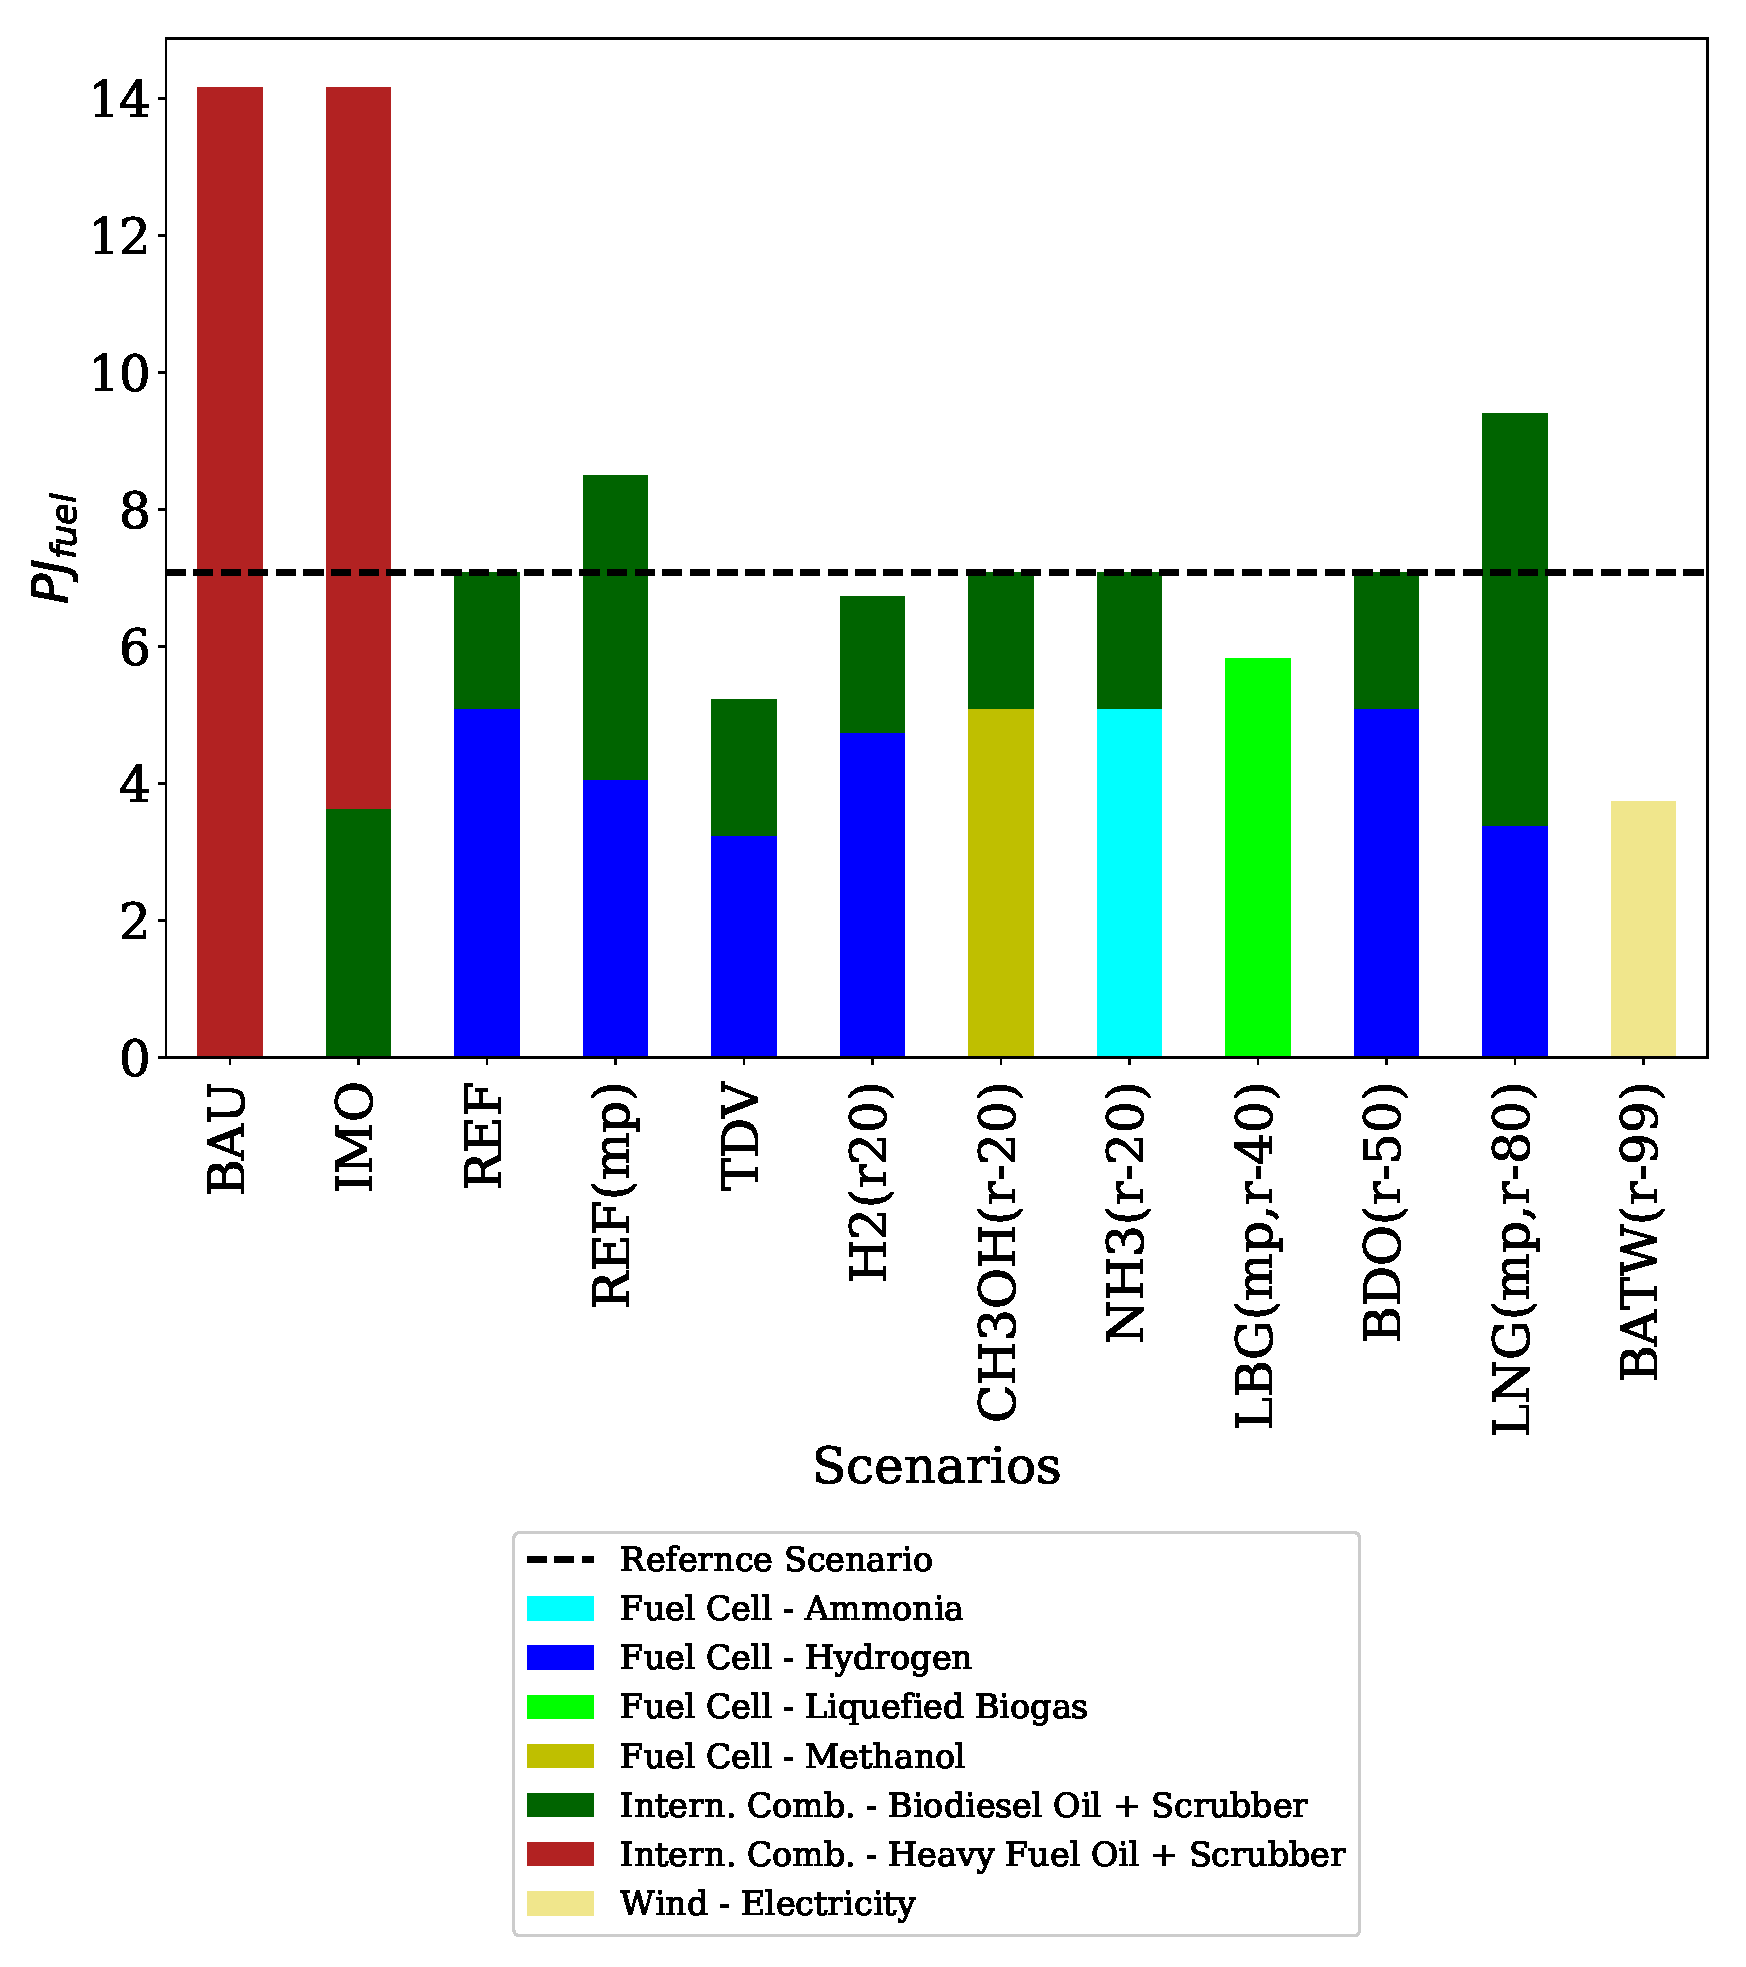
\includegraphics[width=.95\textwidth]{figures/AllFuel2050.eps}
    \label{fig:AllFuel2050}
\end{minipage}\\ %[0.75cm]

Derived from the cost differences for fuel, ship and infrastructure, a carbon price in the range of 350--450 \euro$_{2016}$/ton CO$_2$e would be required for a renewable transition \DIFdelbegin \DIFdel{of }\DIFdelend \DIFaddbegin \DIFadd{to }\DIFaddend the Danish shipping sector. There are no directly comparable studies, but, to put our results in perspective, \citet[p.197]{Raucci2017} reports similar prices of around 430 \$/ton CO$_2$ for a global transition with a global shipping carbon budget \DIFdelbegin \DIFdel{double }\DIFdelend \DIFaddbegin \DIFadd{twice }\DIFaddend as high as in our case. In that setting, he concludes \DIFdelbegin \DIFdel{, }\DIFdelend that hydrogen requires an \DIFdelbegin \DIFdel{emission }\DIFdelend \DIFaddbegin \DIFadd{emissions }\DIFaddend price of 1400 \$/ton CO$_2$ to become an economic option. In contrast, a global study \DIFdelbegin \DIFdel{on }\DIFdelend \DIFaddbegin \DIFadd{of }\DIFaddend country- and sector-wise CO$_2$ abatement costs \cite{OECD2016} \DIFdelbegin \DIFdel{represent }\DIFdelend \DIFaddbegin \DIFadd{represents }\DIFaddend the lower range: \DIFdelbegin \DIFdel{Although }\DIFdelend \DIFaddbegin \DIFadd{although }\DIFaddend shipping is not included, road transport is indicated \DIFdelbegin \DIFdel{with }\DIFdelend \DIFaddbegin \DIFadd{at }\DIFaddend about 200 \euro/ton CO$_2$. Specific costs for climate \DIFdelbegin \DIFdel{emission abatement }\DIFdelend \DIFaddbegin \DIFadd{emission-abatement }\DIFaddend costs in shipping can be expected to be higher than that, since shipping poses special challenges due to \DIFaddbegin \DIFadd{its }\DIFaddend high range requirements. More specifically \DIFdelbegin \DIFdel{on }\DIFdelend \DIFaddbegin \DIFadd{regarding }\DIFaddend CO$_2$ abatement costs for shipping, \citet{DNVGL2017}, assumes costs in the range of 150--200 \euro/avoided ton CO$_2$ if using LBG, methanol based on renewables\DIFaddbegin \DIFadd{, }\DIFaddend or BDO. In reality it can be challenging for a single country to introduce a carbon price on its own\DIFaddbegin \DIFadd{, }\DIFaddend and the analysis should be scaled \DIFdelbegin \DIFdel{to }\DIFdelend \DIFaddbegin \DIFadd{at }\DIFaddend an appropriate level. Thus, the numbers provide an indication of the upper boundary of a necessary worldwide carbon price.

The model code and most of the data references and pre-processing can also be applied \DIFdelbegin \DIFdel{for }\DIFdelend \DIFaddbegin \DIFadd{to }\DIFaddend other countries, especially \DIFaddbegin \DIFadd{in }\DIFaddend Europe. However, since shipping \DIFdelbegin \DIFdel{has a global perspective, the case study for Denmark }\DIFdelend \DIFaddbegin \DIFadd{is global in scope, the Danish case study }\DIFaddend already gives a good indication of the fuel shares chosen for a cost-optimal path to carbon neutrality in 2050 for \DIFdelbegin \DIFdel{the }\DIFdelend worldwide shipping. Conditions for shipping are similar, \DIFaddbegin \DIFadd{as }\DIFaddend the basic parameters, \DIFaddbegin \DIFadd{namely }\DIFaddend technology, fuel and infrastructure costs are considered \DIFdelbegin \DIFdel{as }\DIFdelend \DIFaddbegin \DIFadd{at }\DIFaddend world prices rather than \DIFaddbegin \DIFadd{at prices }\DIFaddend reflecting local particularities. 

Compared to other sectors\DIFaddbegin \DIFadd{, }\DIFaddend like electricity and heat, these mitigation costs per ton \DIFaddbegin \DIFadd{of }\DIFaddend CO$_2$e seem high, but \DIFdelbegin \DIFdel{one has to consider several points }\DIFdelend \DIFaddbegin \DIFadd{several points need to be taken into account}\DIFaddend . First, our results can be interpreted as \DIFdelbegin \DIFdel{the upper bound of cost : Technologies considered are all }\DIFdelend \DIFaddbegin \DIFadd{indicating the upper cost boundary: all potential technologies are considered }\DIFaddend applicable today, \DIFaddbegin \DIFadd{and }\DIFaddend developments in other sectors applying similar technology options could further decrease costs\DIFdelbegin \DIFdel{and additional alternatives could }\DIFdelend \DIFaddbegin \DIFadd{, while additional alternatives might also }\DIFaddend evolve. Second, as shown in the demand reduction scenarios, any decrease in transport demand would save costs even beyond the proportional \DIFdelbegin \DIFdel{saving}\DIFdelend \DIFaddbegin \DIFadd{savings}\DIFaddend . This is due \DIFdelbegin \DIFdel{to not only }\DIFdelend \DIFaddbegin \DIFadd{not only to }\DIFaddend fuel savings (proportional) but \DIFdelbegin \DIFdel{, also due }\DIFdelend \DIFaddbegin \DIFadd{also }\DIFaddend to avoided investments in new ships (disproportionate). A decrease in transport demand especially has an effect in the period, in which new investments in ships are required and  \DIFdelbegin \DIFdel{can thus avoid costs }\DIFdelend \DIFaddbegin \DIFadd{costs can be avoided }\DIFaddend over-proportionally. Note \DIFdelbegin \DIFdel{, that technology }\DIFdelend \DIFaddbegin \DIFadd{that the technological }\DIFaddend progression of renewable energy sources in the electricity sector \DIFdelbegin \DIFdel{have }\DIFdelend \DIFaddbegin \DIFadd{has }\DIFaddend a strong influence on the costs in alternative green shipping (\DIFdelbegin \DIFdel{if }\DIFdelend assuming hydrogen or ammonia). \DIFdelbegin \DIFdel{And third, }\DIFdelend \DIFaddbegin \DIFadd{Third, although }\DIFaddend refits and hybrid solutions have not been considered to \DIFdelbegin \DIFdel{a great extent in the model functionality and could further decrease costs }\DIFdelend \DIFaddbegin \DIFadd{any extent in respect of the model's functionality, they could decrease costs further }\DIFaddend and ease the shift to different fuels.

Transport costs in the BAU scenario amount to roughly 3 \euro$_{2016}$/ton cargo. For climate compatible pathways they are likely to more than double. With \citet[p.~50]{UNCTAD2015} reporting average transport costs of around 5 \euro/ton and including more detail, our results seem to be acceptably precise. Further, \cite[p.~55]{UNCTAD2015} states that transport costs in developed countries are equal to 7 \% of the cargo's import value. Under the assumption of an equal share in \DIFdelbegin \DIFdel{BAU}\DIFdelend \DIFaddbegin \DIFadd{the BAU scenario}\DIFaddend , cargo import values for \DIFdelbegin \DIFdel{the }\DIFdelend climate compatible pathways would increase by 6 -- 8 \%.
Thus, costs could \DIFdelbegin \DIFdel{get lower for }\DIFdelend \DIFaddbegin \DIFadd{fall lower during }\DIFaddend the transition, but the question is also whether \DIFdelbegin \DIFdel{to talk about mitigation costs }\DIFdelend \DIFaddbegin \DIFadd{mitigation costs need to be taken into account}\DIFaddend . Co-benefits like reduced air pollution \DIFdelbegin \DIFdel{have not been }\DIFdelend \DIFaddbegin \DIFadd{were not }\DIFaddend quantified on a monetary basis in the model and were thus not part of the optimisation. However, these could have essential health benefits, maybe even \DIFdelbegin \DIFdel{reaching }\DIFdelend \DIFaddbegin \DIFadd{achieving }\DIFaddend mitigation gains instead of mitigation costs.

The necessary transition will not happen under current market conditions. Regulation is required urgently to bring shipping on \DIFaddbegin \DIFadd{to }\DIFaddend the pathway to carbon neutrality in 2050, in line with the Paris Agreement. A carbon budget for shipping worldwide, broken down \DIFdelbegin \DIFdel{to countries}\DIFdelend \DIFaddbegin \DIFadd{by countries, }\DIFaddend is a viable option to consider. \DIFdelbegin \DIFdel{Additionally}\DIFdelend \DIFaddbegin \DIFadd{In addition}\DIFaddend , more research \DIFdelbegin \DIFdel{for }\DIFdelend \DIFaddbegin \DIFadd{into }\DIFaddend alternative fuels and technologies, as well as solving crucial questions \DIFdelbegin \DIFdel{on }\DIFdelend \DIFaddbegin \DIFadd{regarding issues in respect of }\DIFaddend security, infrastructure and methane leakage\DIFdelbegin \DIFdel{issues are }\DIFdelend \DIFaddbegin \DIFadd{, will be }\DIFaddend important contributions to \DIFdelbegin \DIFdel{implement }\DIFdelend \DIFaddbegin \DIFadd{implementing }\DIFaddend the transition to \DIFdelbegin \DIFdel{climate neutral shipping in }\DIFdelend \DIFaddbegin \DIFadd{climate-neutral shipping by }\DIFaddend 2050. 


\section{Conclusion}
\label{sec:Conclusion}
The achievement of CO$_2$e-neutrality in the shipping sector is of great importance \DIFdelbegin \DIFdel{for reaching }\DIFdelend \DIFaddbegin \DIFadd{if }\DIFaddend the targets of the Paris Agreement \DIFaddbegin \DIFadd{are to be reached}\DIFaddend . Although this goal is underrepresented in the current discussion, this study shows, that it is possible for the Danish \DIFdelbegin \DIFdel{part }\DIFdelend \DIFaddbegin \DIFadd{share }\DIFaddend of international shipping to become CO$_2$e-neutral \DIFdelbegin \DIFdel{until }\DIFdelend \DIFaddbegin \DIFadd{by }\DIFaddend 2050 \DIFdelbegin \DIFdel{with }\DIFdelend \DIFaddbegin \DIFadd{using }\DIFaddend existing technologies. Regarding fuels, \DIFaddbegin \DIFadd{from a socio-economic cost perspective, }\DIFaddend hydrogen, methanol and ammonia are \DIFdelbegin \DIFdel{from a socio-economic cost perspective }\DIFdelend the most compatible\DIFdelbegin \DIFdel{. Due }\DIFdelend \DIFaddbegin \DIFadd{, though due }\DIFaddend to high uncertainties regarding future cost developments and safety requirements (\DIFdelbegin \DIFdel{esp. }\DIFdelend \DIFaddbegin \DIFadd{especially with }\DIFaddend ammonia), there is no clear winner. Regarding technologies, fuel cells are chosen for these fuel options, the decisive parameter being the higher fuel efficiency. Although LNG is the fuel option \DIFdelbegin \DIFdel{most prominently discussed }\DIFdelend \DIFaddbegin \DIFadd{that is discussed most often }\DIFaddend as an alternative today, it would only have a short window of opportunity, mainly because of \DIFdelbegin \DIFdel{leakage problems of methane }\DIFdelend \DIFaddbegin \DIFadd{methane leakage problems }\DIFaddend causing high GHG emissions \DIFdelbegin \DIFdel{, and }\DIFdelend \DIFaddbegin \DIFadd{and the }\DIFaddend high fuel and technology costs. If this gaseous fuel is based on renewable sources, \DIFdelbegin \DIFdel{the }\DIFdelend so-called LBG can only play a role if methane leakage can be drastically reduced \DIFdelbegin \DIFdel{until }\DIFdelend \DIFaddbegin \DIFadd{by }\DIFaddend 2050. The option of \DIFdelbegin \DIFdel{cargo-ships }\DIFdelend \DIFaddbegin \DIFadd{cargo ships being }\DIFaddend driven by a mixture of wind and electricity stored in batteries could not adequately be represented in the model setting\DIFdelbegin \DIFdel{. The evaluation of }\DIFdelend \DIFaddbegin \DIFadd{, an evaluating }\DIFaddend their role would need a further refinement of the calculations. The model itself has \DIFdelbegin \DIFdel{shown }\DIFdelend \DIFaddbegin \DIFadd{proved }\DIFaddend to be a valid tool for assessing pathways for shipping under \DIFdelbegin \DIFdel{emission restriction }\DIFdelend \DIFaddbegin \DIFadd{emission-restriction }\DIFaddend obligations and for assessing the threshold of different fuel options. Although the model has been applied to Danish international shipping, it already gives a good indication of potential fuel shares for worldwide shipping.

The presented modelling approach indicates that either strong \DIFdelbegin \DIFdel{regulative }\DIFdelend \DIFaddbegin \DIFadd{regulatory }\DIFaddend carbon budgets or a carbon price of 350--450 \euro/t~CO$_2$e would be required to induce the necessary changes \DIFdelbegin \DIFdel{for a }\DIFdelend \DIFaddbegin \DIFadd{to achieve }\DIFaddend carbon neutral Danish shipping \DIFdelbegin \DIFdel{in }\DIFdelend \DIFaddbegin \DIFadd{by }\DIFaddend 2050. This would double today's average cargo transport costs. However, due to the low share of transport \DIFdelbegin \DIFdel{cost }\DIFdelend \DIFaddbegin \DIFadd{costs }\DIFaddend on the value of transported goods, the average transported good would only increase by 6 -- 8 \%. This can be considered \DIFdelbegin \DIFdel{as }\DIFdelend the upper limit, since new \DIFdelbegin \DIFdel{fuel possibilities not reflected }\DIFdelend \DIFaddbegin \DIFadd{fuels not represented }\DIFaddend in this study might \DIFdelbegin \DIFdel{evolve}\DIFdelend \DIFaddbegin \DIFadd{be developed}\DIFaddend .

\DIFdelbegin \DIFdel{For }\DIFdelend \DIFaddbegin \DIFadd{In }\DIFaddend the future we perceive \DIFaddbegin \DIFadd{the need and }\DIFaddend potential for more research and development in terms of alternative \DIFdelbegin \DIFdel{green fuel technologies as well as its necessary infrastructureas it remained }\DIFdelend \DIFaddbegin \DIFadd{green-fuel technologies and the necessary infrastructure, as it remains }\DIFaddend uncertain what the exact costs will be\DIFdelbegin \DIFdel{-- pointing out that }\DIFdelend \DIFaddbegin \DIFadd{, though }\DIFaddend some of them \DIFdelbegin \DIFdel{hold }\DIFdelend \DIFaddbegin \DIFadd{have }\DIFaddend great potential and \DIFdelbegin \DIFdel{make it worth to take }\DIFdelend \DIFaddbegin \DIFadd{are worth taking }\DIFaddend a closer look. Moreover, a stronger integration of maritime transport into energy system analysis could highlight \DIFdelbegin \DIFdel{yet idle synergies}\DIFdelend \DIFaddbegin \DIFadd{synergies that are yet still idle}\DIFaddend . Finally, we recommend \DIFdelbegin \DIFdel{to }\DIFdelend \DIFaddbegin \DIFadd{that }\DIFaddend policy makers in this field \DIFdelbegin \DIFdel{to establish clear climate neutral }\DIFdelend \DIFaddbegin \DIFadd{establish clear climate-neutral }\DIFaddend targets for 2050 and \DIFdelbegin \DIFdel{introducing }\DIFdelend \DIFaddbegin \DIFadd{introduc }\DIFaddend the respective measures, preferably \DIFdelbegin \DIFdel{with }\DIFdelend \DIFaddbegin \DIFadd{on }\DIFaddend a broad scale,\DIFdelbegin \DIFdel{e.g. introducing}\DIFdelend \DIFaddbegin \DIFadd{introducing, for example, a tax, a levy or }\DIFaddend an international CO$_2$ quota scheme.


\section*{Acknowledgements}
This work was carried out as part of the FutureGas project (\url{www.futuregas.dk}) financed by the Innovation Fund Denmark [grant number 76084], of which we are grateful. We would \DIFaddbegin \DIFadd{also }\DIFaddend like to thank Niels Tr\ae holt Franck and Thomas Young Hwan Westring Jensen from Energienet and Prof. Olav Hohemeyer (Europa-Universit\"at Flensburg) for very helpful advice during \DIFaddbegin \DIFadd{the }\DIFaddend development and implementation of the model and its application.

\section*{References}
\bibliography{mybibfile}

\newpage
\appendix
\section{Equations}\label{app:equations}
\subsubsection{Nomenclature}\label{box:nomenclature}
\glsdisablehyper
\glsaddall
\begin{table*}[h]
\begin{mdframed}
\footnotesize{
\begin{multicols}{2}
\printglossary[style=tree,type=a]
\vspace{-0.3cm}
\printglossary[style=tree,type=s]
\vspace{-0.3cm}
\printglossary[style=tree,type=v]
\vspace{-0.3cm}
\printglossary[style=tree,type=p]
\end{multicols}
}
\end{mdframed}
\caption*{Nomenclature list.}
\end{table*}

\subsubsection{Objective equation}
The objective equation minimises total system \DIFdelbegin \DIFdel{expenditures }\DIFdelend \DIFaddbegin \DIFadd{expenditure }\DIFaddend over all time steps and ship types (aggregated by main engine and fuel). It comprises the sum of \DIFdelbegin \DIFdel{costs for }\DIFdelend \DIFaddbegin \DIFadd{the costs of }\DIFaddend fuel consumption, additional infrastructure \DIFdelbegin \DIFdel{as well as ship }\DIFdelend \DIFaddbegin \DIFadd{and ships' }\DIFaddend capacity for all years (35 time steps in the described application). \DIFdelbegin \DIFdel{Costs for fixed assets-- }\DIFdelend \DIFaddbegin \DIFadd{The costs of fixed assets, such as }\DIFaddend fuel infrastructure (CI) and ships (CS)\DIFdelbegin \DIFdel{-- are }\DIFdelend \DIFaddbegin \DIFadd{, are are }\DIFaddend given as annuities and \DIFaddbegin \DIFadd{taken into }\DIFaddend account only with the annual added capacities. The value of the existing amount in the start year ($finit_{t,s}$ in $T_0$) is not included in $CI$ \DIFdelbegin \DIFdel{and }\DIFdelend \DIFaddbegin \DIFadd{or }\DIFaddend $CS$.
\begin{subequations}
    \begin{align}
        min. &\sum_{\forall t \in T}\sum_{\forall s \in S}\left( CF_{t, s} + CI_{t, s} + CS_{t, s} \right)\\
        \intertext{subject to (s.t.)}
        CF_{t, s} &\geq f_{t,s} \cdot cf_{t,s}\\
        CI_{t, s} &\geq \left( iup_{t,s} - finit_{t, s} \right) \cdot li_{s} \cdot ci_{t,s}, \forall t \in T_0\\
        CI_{t, s} &\geq iup_{t,s} \cdot li_{s} \cdot ci_{t,s}, \forall t \in T_{>0}\\
        CS_{t, s} &\geq \left( sup_{t,s} - finit_{t, s} \right) \cdot ls_{s} \cdot cs_{t,s}, \forall t \in T_0\\
        CS_{t, s} &\geq sup_{t,s} \cdot ls_{s} \cdot cs_{t,s}, \forall t \in T_{>0}
    \end{align}
\end{subequations}

\subsubsection{Constraints on fuel utilisation, infrastructure and ship capacity}
Fuel constraints may apply \DIFdelbegin \DIFdel{for }\DIFdelend \DIFaddbegin \DIFadd{to }\DIFaddend a selection of ship types and years in the model (\autoref{eq:biofuel}). With regard to infrastructure and ships, only the incremental capacity is cost effective while taking into account \DIFaddbegin \DIFadd{the }\DIFaddend expiry dates of existing capacities. The expiry dates relate to the technical lifetimes, which differ between ships and infrastructure of same type.\\\par\noindent
\textit{Infrastructure capacity: }Defined as the sum of all additional fuel infrastructure built during the elapsed technical lifetime.
\begin{subequations}
    \begin{align}
        icap_{t,s} &\leq \sum_{\textbf{x}}^{t-1} \left( iup_{x,s} \right), \forall t \in T_{>0}, \forall s \in S\label{eq:icap}\\
        \intertext{s.t.}
        x &= T_0, \forall t \leq \left(li_{s} + T_0 - 1\right)\\
        x &= t - li_{s} + 1, \forall t > \left(li_{s} + T_0 - 1\right)
    \end{align}
\end{subequations}\\
\textit{Additional infrastructure: }Additional fuel infrastructure in order to supply the fleet.
\begin{equation}
    iup_{t,s} \geq f_{t,s} - icap_{t,s}, \forall t \in T_{>0}, \forall s \in S\label{eq:iup}
\end{equation}\\
\textit{Existing ships: }Defined as the sum of all additional shipping capacity \DIFdelbegin \DIFdel{build }\DIFdelend \DIFaddbegin \DIFadd{built }\DIFaddend during the elapsed technical lifetime.
\begin{subequations}
    \begin{align}
        scap_{t,s} &\leq \sum_{\textbf{x}}^{t-1} \left(sup_{x,s} \right), \forall t \in T_{>0}, \forall s \in S\label{eq:scap}\\
        \intertext{s.t.}
        x &= T_0, \forall t \leq \left(ls_{s} + T_0 - 1\right)\\
        x &= t - ls_{s} + 1, \forall t > \left(ls_{s} + T_0 - 1\right)
    \end{align}
\end{subequations}\\
\textit{Additional ships: }Additional ships in order to supply the \DIFdelbegin \DIFdel{cargo transport demand}\DIFdelend \DIFaddbegin \DIFadd{demand for cargo transport}\DIFaddend .
\begin{equation}
    sup_{t,s} \geq f_{t,s} - scap_{t,s}, \forall t \in T_{>0}, \forall s \in S\label{eq:sup}
\end{equation}\\
\textit{Refit capacity: }Defines \DIFdelbegin \DIFdel{for each year the old }\DIFdelend \DIFaddbegin \DIFadd{older }\DIFaddend ships' capacity \DIFdelbegin \DIFdel{possible to refit}\DIFdelend \DIFaddbegin \DIFadd{for refitting for each year}\DIFaddend .
\begin{subequations}\label{eq:refitships}
    \begin{align}
    f_{t,s} + f_{t,r} - f_{T_0, s} &\leq 0, \forall t \in T_{<\left(T_0+ls_{s}\right)}, \forall s, r \in SRO\\
    f_{t,s} + f_{t,r} & = 0, \forall t \in T_{\geq\left(T_0+ls_{s}\right)}, \forall s, r \in SRO
    \end{align}
\end{subequations}\\
\textit{Bio-fuel capacity: }Defines \DIFdelbegin \DIFdel{for each year }\DIFdelend the upper limit of bio-fuel available \DIFdelbegin \DIFdel{-- }\DIFdelend \DIFaddbegin \DIFadd{for each year }\DIFaddend based on own assumptions.
\begin{equation}
    \sum_{\forall s \in SB} \left(f_{t,s} \right) - ba_{t}\cdot finit_{T_0} \leq 0, \forall t \in T\label{eq:biofuel}
\end{equation}

\subsubsection{Constraints on transport demand}
\label{subsubsec:tdemand}
\DIFdelbegin \DIFdel{Transport demand constraints may apply for }\DIFdelend \DIFaddbegin \DIFadd{Constraints on the demand for transport may apply to }\DIFaddend a selection of ship types and years in the model, depending on the range category -- either short or long -- and the emission regulations\DIFdelbegin \DIFdel{-- in- or outside emission control }\DIFdelend \DIFaddbegin \DIFadd{, both wthin and outside emission-control }\DIFaddend areas (ECA).\\\par\noindent
\textit{Total transport demand: }Defines for each year that the total transport supply by all ships must be greater or equal to the total transport demand.
\begin{equation}
    dtotal_t \leq \sum_{\forall s \in S} \left( f_{t,s} \cdot sts_{t,s}\right), \forall t \in T \label{eq:td_total}
\end{equation}
\textit{Short transport demand: }Defines for each year the maximum transport supply of all ships categorised as short range (926 km).
\begin{equation}
    dshort_t \geq \sum_{\forall s \in SSR} \left( f_{t,s} \cdot sts_{t,s}\right), \forall t \in T \label{eq:td_short}
\end{equation}
\textit{Non-ECAS transport demand: }Defines for each year the maximum transport supply of all ships only allowed for operation outside of the ECAs.
\begin{equation}
    dnoneca_t \geq \sum_{\forall s \in SNS} \left( f_{t,s} \cdot sts_{t,s}\right), \forall t \in T \label{eq:td_noneca}
\end{equation}

\subsubsection{Constraints on emissions}
\label{subsubsec:emconstraints}
Emission constraints may apply \DIFdelbegin \DIFdel{for }\DIFdelend \DIFaddbegin \DIFadd{to }\DIFaddend a selection of ship types and years in the model. The constraint set imposes limitations \DIFdelbegin \DIFdel{to }\DIFdelend \DIFaddbegin \DIFadd{on }\DIFaddend the deployment of certain fuel types in the model based on the defined CO$_2$e budget and target\DIFaddbegin \DIFadd{, }\DIFaddend as well as the legal restrictions for SO$_X$ and NO$_X$ as defined by the IMO.
\\\par\noindent
\textit{Emission budget: }Defines the maximal amount of accumulated total GHG emissions.
\begin{subequations}
    \begin{align}
    eb &\geq \sum_{\forall t \in T}\sum_{\forall s \in S}\left(EC_{t,s} + EM_{t,s} \right) \label{eq:co2ebudget}\\
    \intertext{s.t.}
    EC_{t,s} &= f_{t,s} \cdot ec_{t,s}, \forall t \in T, \forall s \in S\\
    EM_{t,s} &= f_{t,s} \cdot em_{t,s}, \forall t \in T, \forall s \in S
    \end{align}
\end{subequations}\\
\textit{Emission target: }Defines the amount of GHG emissions allowed in the target year, based on a percentage reduction from the start year.
\begin{equation}
    \frac{\sum_{\forall s \in S} \left(EC_{T_0,s}+EM_{T_0,s}\right)}{\sum_{\forall s \in S} \left(EC_{t,s}+EM_{t,s}\right)} \cdot et \geq 1, \forall t \in T_{\geq \left(tet-T_0\right)}
\end{equation}\\
\textit{Global SO$_X$ regulations: }Defines the set of ships \DIFdelbegin \DIFdel{as of 2020 }\DIFdelend prohibited to operate globally with respect to global SO$_X$ regulations \DIFdelbegin \DIFdel{.
}\DIFdelend \DIFaddbegin \DIFadd{as of 2020.
}\DIFaddend \begin{equation}
    f_{t,s} = 0, \forall t \in T_{\geq teca-T_0}, \forall s \in SNGS \label{eq:sox_global}
\end{equation}\\
\textit{NO$_X$ regulations: }Defines the set of ships \DIFdelbegin \DIFdel{as of 2021 }\DIFdelend prohibited to operate within ECAN \DIFdelbegin \DIFdel{.
}\DIFdelend \DIFaddbegin \DIFadd{as of 2021.
}\DIFaddend \begin{equation}
   f_{t,s} = 0, \forall t \in T_{\geq tneca-T_0},\forall s \in SNN \label{eq:tier}
\end{equation}

\newpage
\section{Tables}
\label{app:tables}
\begin{table}[h]
    \centering
    \resizebox{\textwidth}{!}{
    \begin{tabular}{lrrrrrrrr}
        \toprule
        Fuel type & cf & ci & cf + ci & ec(w2t) & em(w2t) & sulphur content & li & References \\
        & $\left[\frac{EUR_{2016}}{GJ_{fuel}}\right]$ & $\left[\frac{EUR_{2016}}{GJ_{fuel}}\right]$ & $\left[\frac{EUR_{2016}}{GJ_{fuel}}\right]$ & $\left[\frac{g_{CO2}}{MJ_{fuel}}\right]$ & $\left[\frac{g_{CH4}}{MJ_{fuel}}\right]$ & $\left[\%_{mass}\right]$ & $\left[a\right]$ & \\
        \midrule
        HFO   & -        & -        & 6.547     & 8.148         & 0.090            & 2.9525   & 40   & \cite{BIX2018,Gilbert2018,Bengtsson2012,BRYNOLF2014}    \\
        MDO   & -        & -        & 12.775    & 7.728         & 0.090            & 0.7500   & 40   & \cite{BIX2018,Gilbert2018,Bengtsson2012,Andersson2015}    \\
        BDO   & -        & -        & 24.240    & 0             & 0.030            & 0.1498   & 40   & \cite{SSI2018,Bengtsson2012}    \\
        LNG   & 4.888    & 0.139    & -         & 6.600         & 0.033            & 0.0500   & 36   & \cite{EnerginNet2018,Gilbert2018,BRYNOLF2014,Andersson2015}    \\
        LBG   & 27.847   & 1.599    & -         & 0             & 0.130            & 0.0750   & 25   & \cite{Brynolf2018,Bengtsson2012}    \\
        H2    & 20.885   & 1.199    & -         & 0             & 0                & 0        & 25   & \cite{Brynolf2018}    \\
        CH3OH & 29.240   & 1.679    & -         & 0             & 0.042            & 0.0912   & 25   & \cite{Brynolf2018,BRYNOLF2014}    \\
        NH3   & 26.803   & 1.802    & -         & 0             & 0                & 0        & 20   & \cite{Morgan2017}    \\
        ELEC  & 13.889   & 2.929    & -         & 0             & 0                & 0        & 20   & \cite{Vree2008}    \\
        \bottomrule
    \end{tabular}}
    \caption[Fuel type data]{Fuel type data for each parameter (for abbreviations see the nomenclature list in \ref{box:nomenclature}). Further explanation \DIFdelbeginFL \DIFdelFL{of }\DIFdelendFL \DIFaddbeginFL \DIFaddFL{to }\DIFaddendFL data can be found in \cite{Thesis2018}.}
    \label{tab:fuel_data}
\end{table}
\begin{table}[h]
    \centering
    \resizebox{\textwidth}{!}{
    \begin{tabular}{llrrrrrrrrrrr}
        \toprule
                       Ship-type & Range & ls & fa$_{2016}$ & ts & cs & ec(t2p) & em(t2p) & Refit & Refit opt. & Tier & Scrubber & References \\
                       &       & $\left[a\right]$ & $\left[PJ_{fuel}\right]$ & $\left[\frac{Ttkm}{GJ_{fuel}}\right]$ & $\left[\frac{EUR_{2016}}{GJ_{fuel}}\right]$ & $\left[\frac{g_{CO2}}{MJ_{fuel}}\right]$ & $\left[\frac{g_{CH4}}{MJ_{fuel}}\right]$ & & & & & \\
        \midrule
        IC HFO (old)   & long  & 11     & 9.93   & 9.69        & 8.72     & 76.06            & 0.00045          & yes   & IC HFO (refit) & 0           & no     & \cite{UNCTAD2017,Eurostat2018,Wisdom2017,Kristensen2012,Rex2017} \\
        IC MDO (old)   & long  & 11     & 5.99   & 9.40        & 8.45     & 74.36            & 0.00045          & yes   & IC BDO (refit) & 0           & yes    & \cite{UNCTAD2017,Eurostat2018,Wisdom2017,Kristensen2012,Rex2017} \\
        IC HFO         & long  & 25     & 0      & 9.40        & 8.45     & 75.90            & 0.00045          & no    & -              & 3           & yes    & \cite{UNCTAD2017,Kristensen2012,Rex2017} \\
        IC MDO         & long  & 25     & 0      & 9.40        & 8.45     & 74.32            & 0.00045          & no    & -              & 3           & yes    & \cite{UNCTAD2017,Kristensen2012,Rex2017} \\
        IC HFO (refit) & long  & 11     & 0      & 9.40        & 0.02     & 75.90            & 0.00045          & no    & -              & 3           & yes    & \cite{UNCTAD2017,McGill2013} \\
        IC BDO (refit) & long  & 11     & 0      & 9.40        & 0        & 0                & 0.00045          & no    & -              & 3           & yes    & \cite{UNCTAD2017,Wisdom2017} \\
        IC BDO         & long  & 25     & 0      & 9.40        & 8.45     & 0                & 0.00045          & no    & -              & 3           & yes    & \cite{UNCTAD2017,Bengtsson2012} \\
        IC LNG         & long  & 25     & 0      & 10.13       & 96.98    & 54.36            & 0.71000          & no    & -              & 3           & no     & \cite{UNCTAD2017,Kristensen2012,Rex2017} \\
        IC LBG         & long  & 25     & 0      & 10.13       & 96.98    & 0                & 0.79000          & no    & -              & 3           & no     & \cite{UNCTAD2017,Bengtsson2012} \\
        IC H2          & long  & 25     & 0      & 10.13       & 109.29   & 0                & 0                & no    & -              & 3           & no     & \cite{UNCTAD2017,ElGohary2013} \\
        IC CH3OH       & long  & 25     & 0      & 10.13       & 109.29   & 0                & 0.79000          & no    & -              & 3           & no     & \cite{UNCTAD2017,Andersson2015,BRYNOLF2014} \\
        IC NH3         & long  & 25     & 0      & 10.13       & 109.29   & 0                & 0                & no    & -              & 3           & no     & \cite{UNCTAD2017} \\
        FC LNG         & long  & 25     & 0      & 22.47       & 134.80   & 54.36            & 0.22763          & no    & -              & 3           & no     & \cite{UNCTAD2017,VanBiert2016} \\
        FC LBG         & long  & 25     & 0      & 22.47       & 134.80   & 0                & 0.22763          & no    & -              & 3           & no     & \cite{UNCTAD2017,VanBiert2016} \\
        FC H2          & long  & 25     & 0      & 22.47       & 134.80   & 0                & 0                & no    & -              & 3           & no     & \cite{UNCTAD2017,USDE2015} \\
        FC CH3OH       & long  & 25     & 0      & 22.47       & 134.80   & 0                & 0.22763          & no    & -              & 3           & no     & \cite{UNCTAD2017,VanBiert2016} \\
        FC NH3         & long  & 25     & 0      & 22.47       & 134.80   & 0                & 0                & no    & -              & 3           & no     & \cite{UNCTAD2017} \\
        EM ELEC        & short & 30     & 0      & 11.86       & 1,047.05 & 0                & 0                & no    & -              & 3           & no     & \cite{DNVGL2015} \\
        WIND ELEC      & long  & 30     & 0      & 35.58       & 2,094.11 & 0                & 0                & no    & -              & 3           & no     &  \\  
    \bottomrule
    \end{tabular}}
    \caption[Ship type data]{Ship type data for each specific parameter (for abbreviations see the nomenclature list in \ref{box:nomenclature}). Further explanation and references of data can be found in \cite{Thesis2018}.}
    \label{tab:ship_data}
\end{table}
\begin{table}[t]
    \centering
    \resizebox{\textwidth}{!}{%
    \begin{tabular}{lrlr}
        \toprule
        Modified & Percentage & Affected Technologies & References \\
        para- & change & & \\
        meters & 2016-2050 & & \\
        \midrule
        ic  & -20           & LNG,LBG,H2,CH3OH,NH3,ELEC                         & \cite[fig.~6,~p.~13]{Brynolf2018}     \\[1.5ex]
        \multirow{2}{*}{cf} & 110   & HFO,MDO,BDO,LNG                           & \cite[fig.~13,~p.~3]{JAE-KNY/MDA2017} \\
            & -20           & LBG,H2,CH3OH,NH3,ELEC                             & \cite[fig.~6,~p.~13]{Brynolf2018}     \\[1.5ex]
        \multirow{2}{*}{cs} & -40   & Internal combustion: LNG,LBG,H2,CH3OH,NH3 & \cite{Rex2017}                        \\
            & -50           & Fuel cell: LNG,LBG,H2,CH3OH,NH3                   & \cite{Rex2017}                        \\
            & -75           & Eletric motor, WIND: ELEC                         & \cite{Rex2017}                        \\[1.5ex]
        ts  & +15           & All except old ships                              & \cite[tab.~51,~p.~282]{Smith2014}     \\[1.5ex]
        ec  & -10           & IC: HFO,MDO,LNG; FC: LNG                          & \cite[tab.~51,~p.~282]{Smith2014}     \\[1.5ex]
        em  & -10           & IC: HFO,MDO,BDO,LNG; FC: LNG,LBG                  & \cite[tab.~51,~p.~282]{Smith2014}     \\
        \bottomrule
    \end{tabular}}
    \caption{Change of fuel and ship specific parameters from 2016 to 2050 in the Reference scenario (for abbreviations see the nomenclature list in \ref{box:nomenclature}).For additional information about scenarios see \cite{Thesis2018}.}
    \label{tab:ref_rates}
\end{table}

\clearpage
\section{Figures}
\begin{figure}[h]
    \centering
    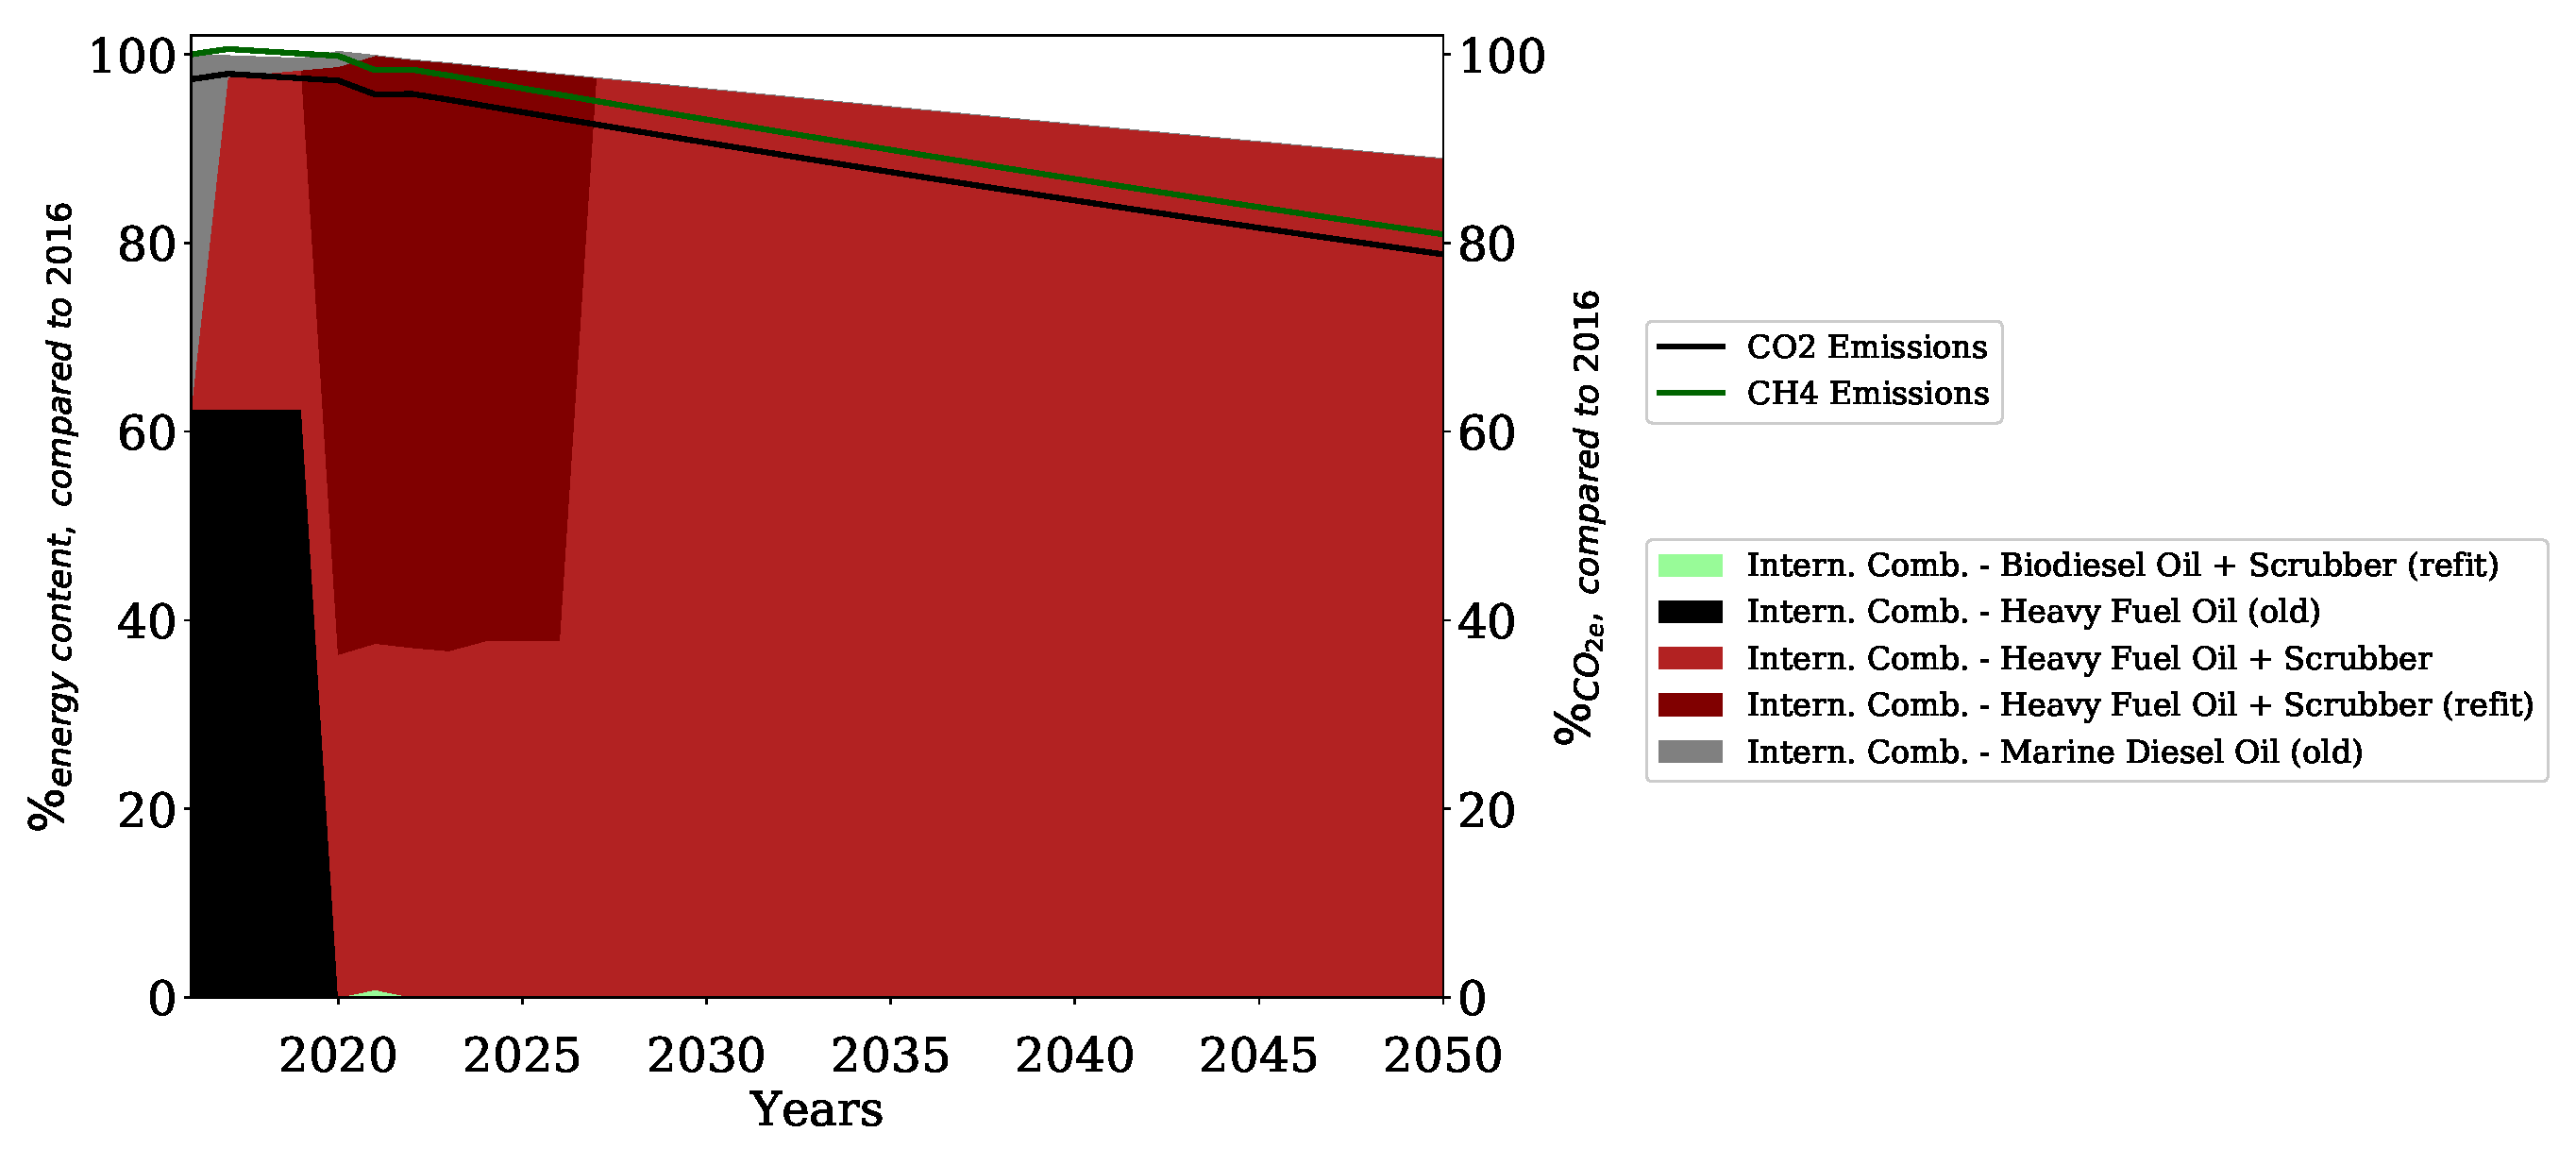
\includegraphics[width=\textwidth]{figures/BAU_fuels_emissions.eps}
    \caption{Fuel consumption (y-axis left) and cumulative emissions (y-axis right) in the business-as-usual scenario without carbon restrictions.}
    \label{fig:BAU}
\end{figure}
\begin{figure}[h]
    \centering
    \includegraphics[width=\textwidth]{figures/TDVAR_fuels_emissions.eps}
    \caption{Fuel consumption (y-axis left) and cumulative emissions (y-axis right) in the reduced transport demand scenario with a limited carbon budget and assuming methane leakage phase-out.}
    \label{fig:TDV}
\end{figure}
\begin{figure}[h]
    \centering
    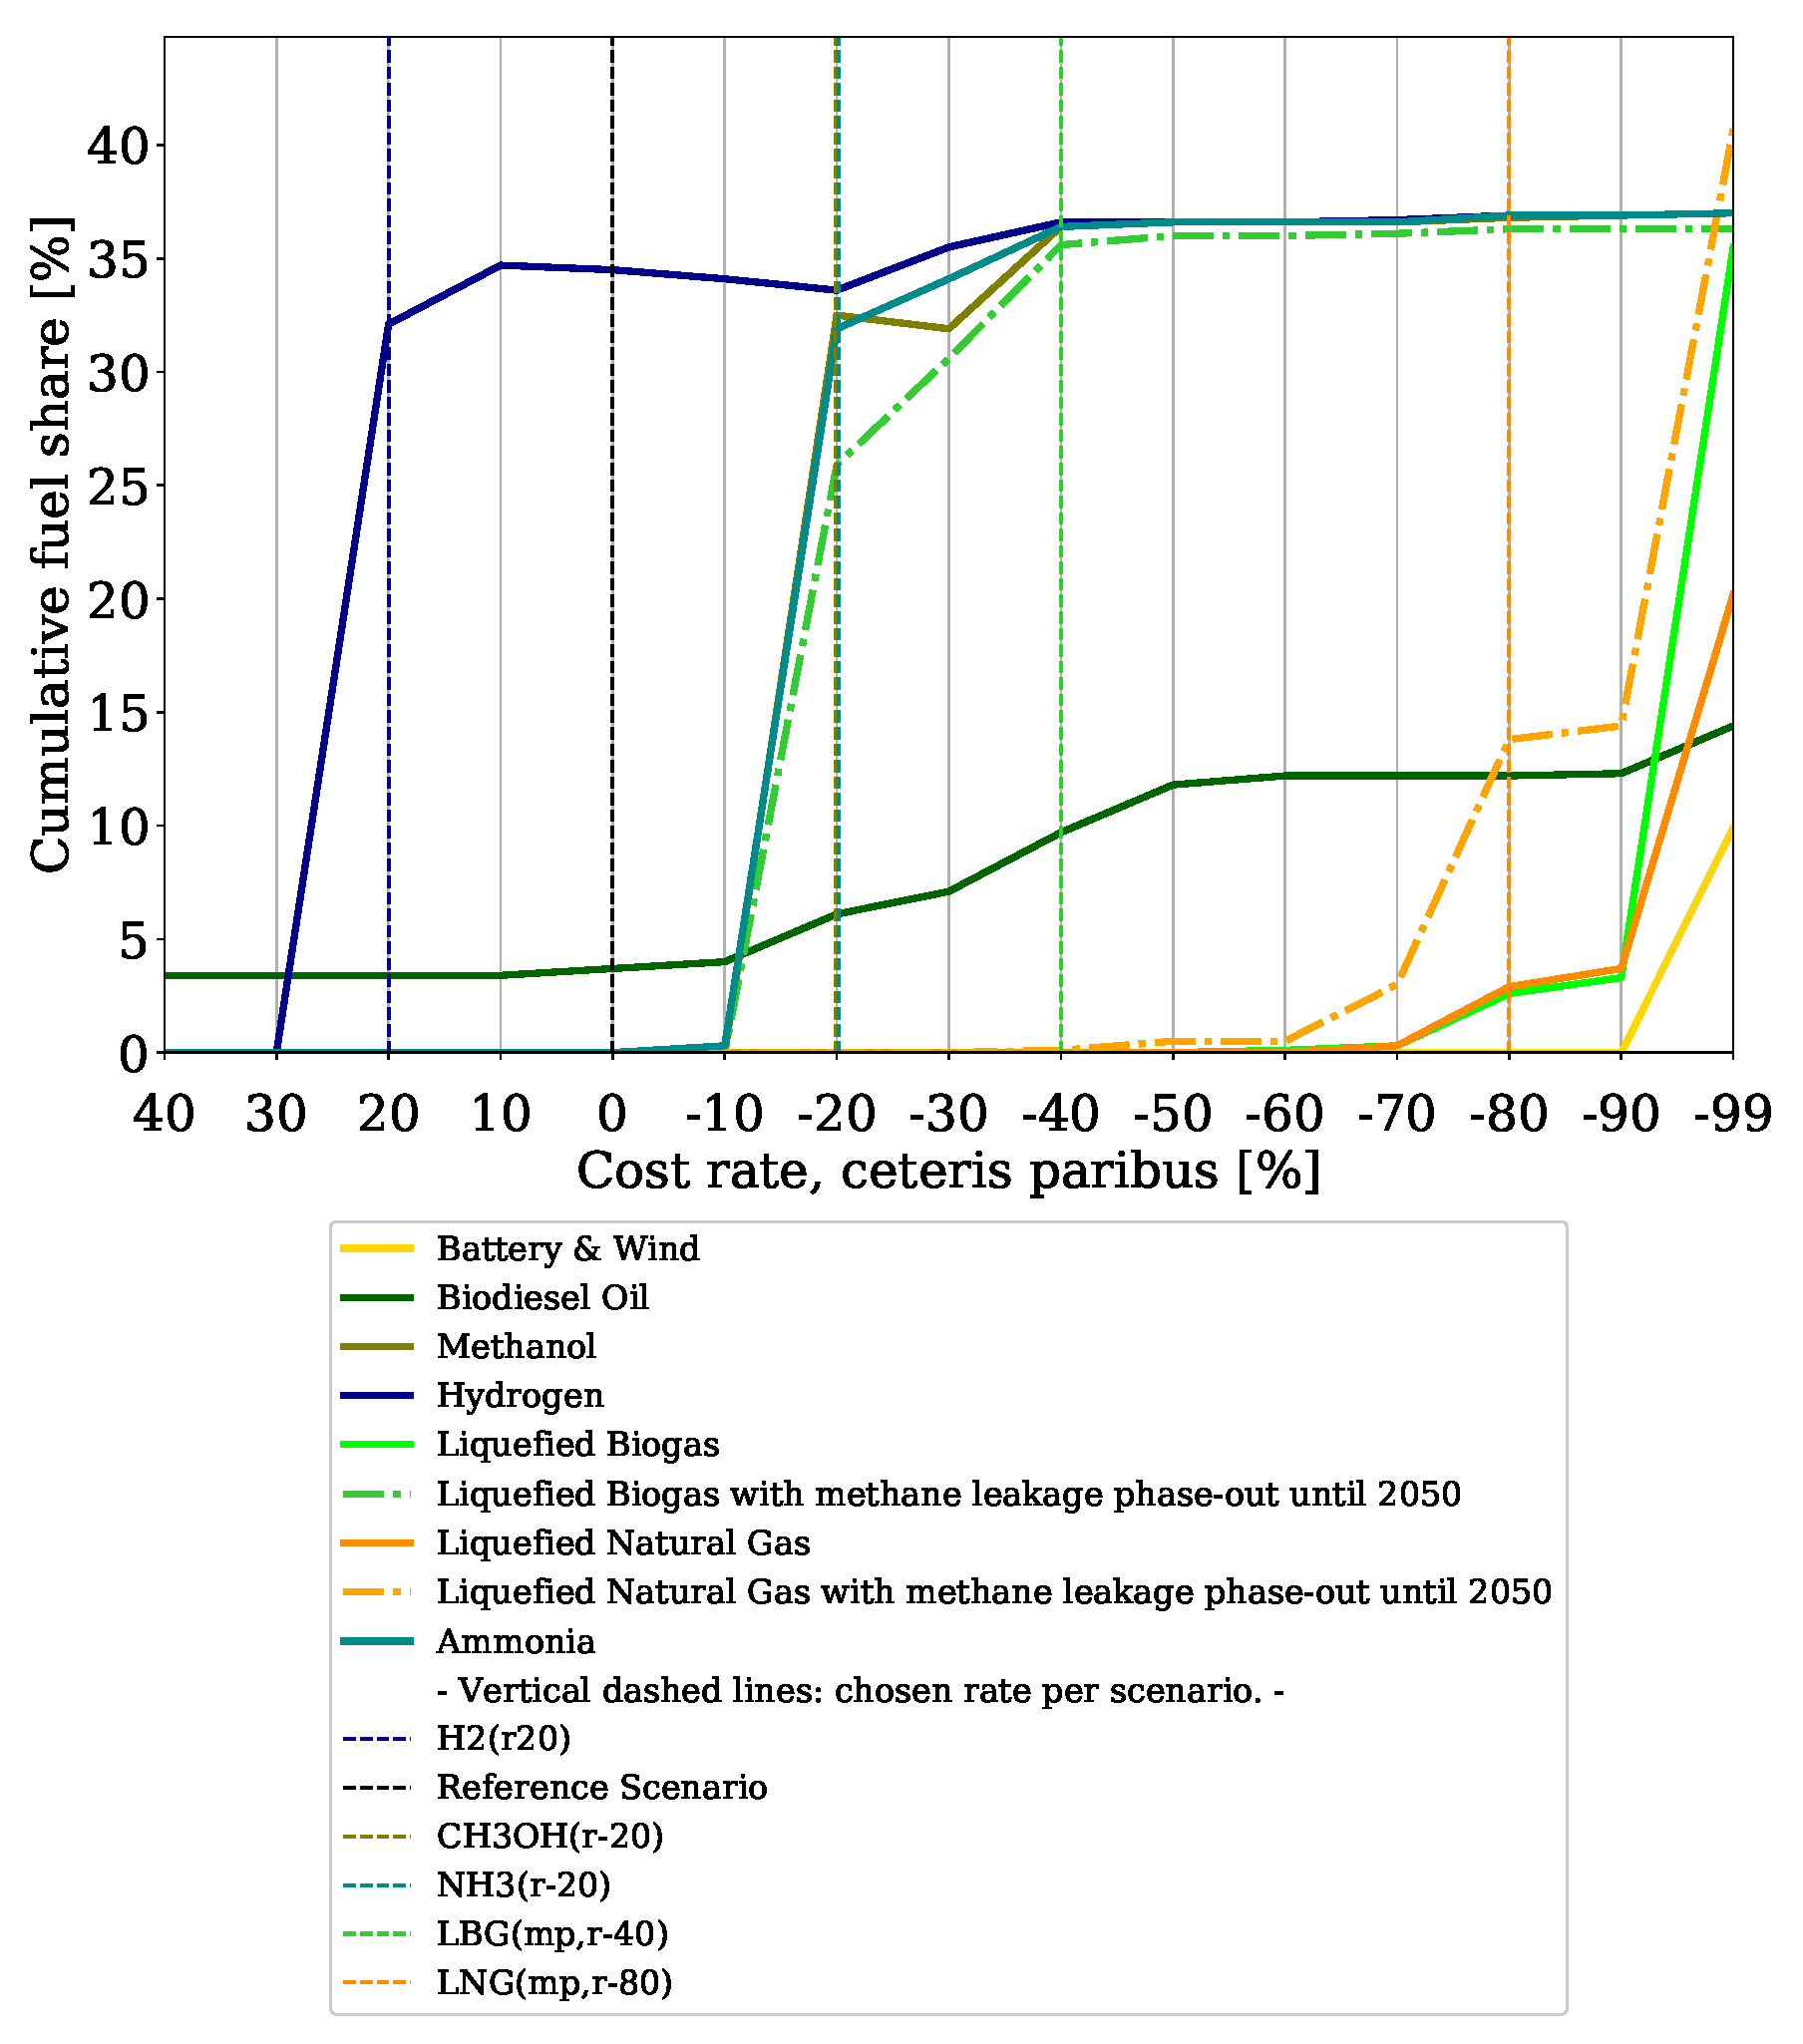
\includegraphics[width=.825\textwidth]{figures/costVariation.eps}
    \caption{Total fuel shares from 2016-2050 (y-axis) in relation to different cost range changes (x-axis) compared to the reference case.}
    \label{fig:costVariation}
\end{figure}
\begin{figure}[h]
    \centering
    \includegraphics[width=\textwidth]{figures/LBG_MP_fuels_emissions.eps}
    \caption{Fuel consumption (y-axis left) and cumulative emissions (y-axis right) in the bio-methane scenario (LBG(mp), r-40) and assuming methane leakage phase-out.}
    \label{fig:LBG}
\end{figure}

\end{document}